 %
% exemplo genérico de uso da classe iiufrgs.cls
% $Id: iiufrgs.tex,v 1.1.1.1 2005/01/18 23:54:42 avila Exp $
%
% This is an example file and is hereby explicitly put in the
% public domain.
%
\documentclass[ppgc,tese, english]{iiufrgs}
% Para usar o modelo, deve-se informar o programa e o tipo de documento.
% Programas :
%   * cic       -- Graduação em Ciência da Computação
%   * ecp       -- Graduação em Ciência da Computação
%   * ppgc      -- Programa de Pós Graduação em Computação
%   * pgmigro   -- Programa de Pós Graduação em Microeletrônica
%   
% Tipos de Documento:
%   * tc                -- Trabalhos de Conclusão (apenas cic e ecp)
%   * diss ou mestrado  -- Dissertações de Mestrado (ppgc e pgmicro)
%   * tese ou doutorado -- Teses de Doutorado (ppgc e pgmicro)
%   * ti                -- Trabalho Individual (ppgc e pgmicro)
% 
% Outras Opções:
%   * english    -- para textos em inglês
%   * openright  -- Força início de capítulos em páginas ímpares (padrão da
%                   biblioteca)
%   * oneside    -- Desliga frente-e-verso
%   * nominatalocal -- Lê os dados da nominata do arquivo nominatalocal.def

\usepackage{amsmath,amssymb,amsfonts}
\usepackage{amsmath}
\usepackage{siunitx}
\usepackage{textgreek}
\usepackage{booktabs}
\usepackage{multirow}
\usepackage{lscape}
\usepackage{tabularx}
\usepackage{ltablex} 
\usepackage{arydshln}
\usepackage{lettrine}
\usepackage[thinlines]{easytable}
\usepackage{hhline}

% Use unicode
\usepackage[utf8]{inputenc}   % pacote para acentuação

% Necessário para incluir figuras
\usepackage{graphicx}           % pacote para importar figuras
\usepackage{subcaption}
\usepackage{mathtools}
\captionsetup{compatibility=false}

\usepackage{times}              % pacote para usar fonte Adobe Times
% \usepackage{palatino}
% \usepackage{mathptmx}          % p/ usar fonte Adobe Times nas fórmulas

\usepackage[alf,abnt-emphasize=bf]{abntex2cite}	% pacote para usar citações abnt

\definecolor{myred}{RGB}{255, 0, 0}

\hyphenation{ro-bo-tics}
\hyphenation{method-olo-gies}
\hyphenation{wheth-er}
\DeclareMathOperator*{\argmax}{arg\,max}
\DeclareMathOperator*{\argmin}{arg\,min}
\newcommand{\bs}{\boldsymbol}
\newcommand{\comment}[1]{}
%
% Informações gerais
%
\title{Exploiting organisational semantic information in indoor environments for the object search problem}

\author{Mantelli}{Mathias Fassini}
% alguns documentos podem ter varios autores:
%\author{Flaumann}{Frida Gutenberg}
%\author{Flaumann}{Klaus Gutenberg}

% orientador e co-orientador são opcionais (não diga isso pra eles :))
\advisor[Profa.~Dra.]{Kolberg}{Mariana Luderitz}
\coadvisor[Prof.~Dr.]{Maffei}{Renan de Queiroz}

% a data deve ser a da defesa; se nao especificada, são gerados
% mes e ano correntes
%\date{maio}{2001}

% o local de realização do trabalho pode ser especificado (ex. para TCs)
% com o comando \location:
%\location{Itaquaquecetuba}{SP}

% itens individuais da nominata podem ser redefinidos com os comandos
% abaixo:
% \renewcommand{\nominataReit}{Prof\textsuperscript{a}.~Wrana Maria Panizzi}
% \renewcommand{\nominataReitname}{Reitora}
% \renewcommand{\nominataPRE}{Prof.~Jos{\'e} Carlos Ferraz Hennemann}
% \renewcommand{\nominataPREname}{Pr{\'o}-Reitor de Ensino}
% \renewcommand{\nominataPRAPG}{Prof\textsuperscript{a}.~Joc{\'e}lia Grazia}
% \renewcommand{\nominataPRAPGname}{Pr{\'o}-Reitora Adjunta de P{\'o}s-Gradua{\c{c}}{\~a}o}
% \renewcommand{\nominataDir}{Prof.~Philippe Olivier Alexandre Navaux}
% \renewcommand{\nominataDirname}{Diretor do Instituto de Inform{\'a}tica}
% \renewcommand{\nominataCoord}{Prof.~Carlos Alberto Heuser}
% \renewcommand{\nominataCoordname}{Coordenador do PPGC}
% \renewcommand{\nominataBibchefe}{Beatriz Regina Bastos Haro}
% \renewcommand{\nominataBibchefename}{Bibliotec{\'a}ria-chefe do Instituto de Inform{\'a}tica}
% \renewcommand{\nominataChefeINA}{Prof.~Jos{\'e} Valdeni de Lima}
% \renewcommand{\nominataChefeINAname}{Chefe do \deptINA}
% \renewcommand{\nominataChefeINT}{Prof.~Leila Ribeiro}
% \renewcommand{\nominataChefeINTname}{Chefe do \deptINT}

% A seguir são apresentados comandos específicos para alguns
% tipos de documentos.

% Relatório de Pesquisa [rp]:
% \rp{123}             % numero do rp
% \financ{CNPq, CAPES} % orgaos financiadores

% Trabalho Individual [ti]:
% \ti{123}     % numero do TI
% \ti[II]{456} % no caso de ser o segundo TI

% Monografias de Especialização [espec]:
% \espec{Redes e Sistemas Distribuídos}      % nome do curso
% \coord[Profa.~Dra.]{Weber}{Taisy da Silva} % coordenador do curso
% \dept{INA}                                 % departamento relacionado

%
% Palavras-chave
% A primeira palavra de cada palavra-chave (que, ironicamente, pode ser várias palavras) deve sempre
% começar em maíuscula (novo padrão da biblioteca), as demais palavras começam em minúscula, exceto
% se são nomes próprios.
%
\keyword{Mobile robotics}
\keyword{Object search}
\keyword{Organisational semantic information}
\keyword{Robotics perception}
\keyword{Indoor environments}


%
% inicio do documento
%
\begin{document}

% folha de rosto
% às vezes é necessário redefinir algum comando logo antes de produzir
% a folha de rosto:
% \renewcommand{\coordname}{Coordenadora do Curso}
\maketitle

% DEDICATORIA
%Entre os mais fortes existem os que nasceram com um dom, e aqueles que trabalham duro… E eu sou um dos que trabalhou duro!”, Rock Lee
%
\clearpage
\begin{flushright}
\mbox{}\vfill
{\sffamily\itshape
``You are seeking happiness.\\
Learn this lesson, once and forever,\\
that you will find happiness only by\\
helping others to find it!''\\}
--- \textsc{Outwitting the Devil}
\end{flushright}

% AGRADECIMENTOS
\chapter*{Acknowledgements}
My supervisors Prof. Mariana Kolberg and Prof. Renan Maffei have been endless sources of guidance during all these years. I have been under Prof. Mariana's supervision since I was a master's degree student, and I have grown and learned immensely since then. I am thankful for the two opportunities she gave me to learn not just about Mobile Robotics but many other exciting topics. Prof. Renan has been my co-supervisor even before becoming a professor, when he was still a PhD candidate at Phi Group. I have always admired him for his skills, critical thinking and out of the box ideas. His passion for Phi Group and his dedication have motivated me to do the same during these years. It was with their supervision that this work came into existence. Thank you for the excellent cooperation and for all of the opportunities I was given to, besides boosting my technical skills, broaden my personal horizons during this incredibly instructive period. Besides, I would like to thank Prof. Edson Prestes, head of Phi Group, for the moments we shared in the lab and for how much he taught me throughout these years.

I would like to thank Prof. Jim Torresen for receiving me at his ROBIN lab in Norway. This opportunity to live abroad and exchange knowledge with other researchers was essential for me as a PhD candidate, and I am thankful for that. Many thanks go also to the ROBIN members for the great time I had in the group. 

Many special thanks to two international friends, Robin Weiss and Sadegh Hosseinpoor. Robin has not only helped me to grow personally with great conversations about essential aspects of life, but he also has encouraged me to study and live abroad until it came true. I should thank him for always believing in me. Our road trip through Europe was a memorable adventure, and it changed my life. Sadegh has been a special friend for a long time, and we had great moments in Norway that I will not forget. My life experience in Norway would be way more challenging without our volleyball training sections, pool games, and camping adventures. 

I should also thank the members of Phi Group for the great time I had in our group. I enjoyed the atmosphere and their support. A special thank goes to a close friend Diego Pittol. He has been a partner in crime since my master's, and I have learned a lot with him. Our discussions and his attention to every detail contributed to completing this thesis. I would not be able to go through this unique adventure without him. I thank him for everything he has done for me, mainly for taking care of me during the challenging moments of my life. 

Additionally, I wish to thank my family, Vadirlei, Luiza, Fabiane, and Marcelo, who have always supported me and lovingly understood my absence during special moments. I also would like to express my gratitude to Fernanda for her unconditional support over the past two years and for enjoying life together with me. 

My PhD course has been a long journey that has taken me to many places, where I had the great opportunity to meet, collaborate, work, and have fun with amazing people. It is impossible to sum up years of experience and interaction with all of them, but I am sure they already know how awesome I think they are. Hence, I made this instead. 

%\begin{figure}[!h]
%\centering
\vspace{.5cm}\hspace{1.6cm}\includegraphics[width=.65\textwidth]{figs/acknowledgment.png}
%\caption{}
%\end{figure}

%I would like to thank Professor Peter Glösekötter, who has been supportive since the days I was an undergraduate student, and whose drive for innovation I admire. It was with his supervision that this work came into existence. In addition to my stay in Brazil, he enabled me to both work and pursue my studies in England, Spain, and China. Thank you for the excellent cooperation and for all of the opportunities I was given to, besides boosting my technical skills, broaden my personal horizons during this incredibly instructive period.

%Also, I must express my sincere gratitude to Mariana Kolberg and Edson Prestes for co-supervising this work. Thank you for the lively discussions and your patient mentoring. Collaborating with you and the whole team of the Φ-Robotics Research Group has enriched my experience in Porto Alegre tremendously. I have been extremely lucky to have been surrounded by people like you, who cared so much about my work and who responded to my questions and queries so promptly.

%My wholehearted gratefulness and appreciation goes to Mathias Mantelli, who helped me grow personally beyond my work at the keyboard and who cheered me up during the most difficult times when writing this thesis. Without him, I would have been lost many times. Our stimulating discussions and his attention to detail profoundly contributed in the completion of this thesis. Thank you for all the fun we had in the past six months.

%I heartily dedicate this thesis to my mother Karin and to my brother Manuel, whose love and guidance are with me in whatever I pursue. Thank you for providing me with unfailing support and continuous encouragement throughout my years of study and through the process of researching and writing this thesis. What I have accomplished would not have been possible without you.

%Last but not least, I would like to express my very profound gratitude to my friends Nina, Denise, Sebastian and Tim. I am so blessed to have you by my side. During all the months-long periods that I spent abroad, you were the ones who waited patiently for me to return whilst encouraging me from back home. 

%Thank you all for your unwavering support.


% Resumo na língua do documento.
\begin{abstract}
Nowadays, the mobile robotics research community deals with different high-level tasks that require the robot to manipulate or interact with objects that may not be in the robot's field of view. To find an object in unknown environments, the robot needs to look for it while gaining information about the environment and making decisions in real-time, known as the object search (OS) problem. The research community has proposed different approaches for dealing with the OS problem, relying on the objects' color or 3D shape as visual cues to guide the search. However, this geometric information (i.e., color or size) limits the robot's perception and, consequently, the robot's performance during the search. Therefore, we propose two OS systems that exploit the advantages of semantic information inferred from the organisation of both the environment and objects. The first one relies on semantic information inferred from numbers in text signs found in the environment. The goal is to find a target door label. The use of organisational semantic information in this scenario allows the robot to reduce the search costs by avoiding not promising corridors to contain the target door label. The detected numbers are used to estimate either the search continues towards unknown parts of the environment, or carefully search in the already known parts. The second proposed OS system is based on the changes in the organisation and arrangement of objects over time in the environment. It observes the environment and gathers data from the objects' placement through the time by executing its recording mode. This recorded data is later used when the robot executes the requesting mode to search for the target object. Both systems were evaluated in different environments and compared against other OS approaches in simulated and real scenarios. The results support our systems' efficiency and demonstrate the improvement in the searching performance with the aid of organisational semantic information.
\end{abstract}

% Resumo na outra língua, se o documento estiver em português, esse estará em inglês,
% se o documento estiver em inglês, este deve estar em português.
% Devem ser passados como parâmetros: o título e as palavras-chave
% na outra língua, separadas por pontos, sem ponto após a última palavra-chave.
% O mesmo padrão de capitalizar a primeira palavra de cada palavra-chave deve ser seguido aqui.
% Seguindo a ideia de não traduzir nomes próprios, nem UFRGS, nem ABNT, nem "Instituto de Informática
% da UFRGS" são traduzidos.
\begin{englishabstract}{Explorando Informações Semânticas em Ambientes Internos}{Robótica móvel. Busca por objectos. Informação semântica. Percepção robótica. Ambientes internos}
Atualmente, a comunidade científica de robótica móvel está lidando com diferentes tarefas de alto-nível que requerem que o robô manipule ou interaja com objetos que podem não estar no campo de visão do robô. Para encontrar um objeto em um ambiente desconhecido, o robô precisa procurar por ele enquanto ganha informação sobre o ambiente e toma decisões em tempo-real, conhecido como o problema de busca por objetos (BPO). A comunidade de pesquisa propôs diferentes soluções para abordar o problema de BPO, se baseando na cor, tamanho ou no que existe ao redor dos objetos. Contudo, todas essas informações geométricas (como por exemplo cor ou tamanho) limita a percepção do robô e, por consequência, o seu desempenho durante a busca. Portanto, nós propomos dois sistemas de BPO que exploraram as vantagens de informações semânticas inferidas a partir da organização tanto do ambiente quanto dos objetos presentes. O primeiro se baseia em informações semânticas inferidas de números em placas de texto encontrados no ambiente. O objetivo é encontrar a placa de texto da porta alvo. O uso da informação semântica organizacional neste cenário permite que o robô reduza os custos da busca por evitar corredores não promissores para conter a placa de texto da porta alvo. Os números detectados são usados para estimar se busca continua em direção a regiões desconhecidas ou se realiza a busca cuidadosamente em regiões já conhecidas. O segundo sistema de BPO é baseado nas mudanças na organização e arranjo dos objetos ao longo do tempo no ambiente. Nosso sistema observa o ambiente e coleta dados do posicionamento dos objetos ao longo do tempo executando o seu modo de gravação. Os dados gravados são usados posteriormente quando o robô executa o modo de requisição para buscar pelo objeto. Ambos os sistemas foram avaliados em diferentes ambientes e comparados contra outros sistemas de BPO em simulação e ambiente real. Os resultados confirmam a eficiência dos nossos sistemas e demonstram a melhora no desempenho da busca com o auxílio das informações semânticas organizacional.
\end{englishabstract}

% lista de figuras
\listoffigures

% lista de tabelas
\listoftables

% lista de abreviaturas e siglas
% o parametro deve ser a abreviatura mais longa
% As abreviações devem estar em ordem alfabética (levando em conta só a abreviação mesmo,
% não o que significa cada palavra).
\begin{listofabbrv}{SPMD}
        \item[BVP] Boundary Value Problem
        \item[DS] Door Simulator        
        \item[DSR] Domestic Service Robot
        \item[ER] Extremal Region
        \item[FoV] Field of View
        \item[FPS] Frames per Second
%        \item[GPS] Global Positioning System
        \item[HIMM] Histogram In-Motion Mapping                
        \item[IFR] International Federation of Robotics
 %       \item[IR] Industrial Robot
        \item[KDE] Kernel Density Estimation
        \item[MCL] Monte Carlo Localization
        \item[OCR] Optical Character Recognition
        \item[OS] Object Search
        \item[PD] Population Division
        \item[PSR] Professional Service Robot
        \item[RBPF] Rao-Blackwellized Particle Filter
        \item[RGB] Red, Green, Blue
        \item[RGB-D] Red, Green, Blue, Depth                        
%        \item[RIA] Robotic Industries Association
%        \item[ROI] Region of Interest
        \item[SARS-CoV-2] ~~~~~~~~~~~~~~Severe Acute Respiratory Syndrome Coronavirus 2
        \item[SLAM] Simultaneous Localization and Mapping
        \item[SR] Service Robot        
        \item[UAV] Unmanned Aerial Vehicle
        \item[YOLO] You Only Look Once
        
\end{listofabbrv}

% idem para a lista de símbolos
\begin{listofsymbols}{$\alpha\beta\pi\omega$}
	\item [$\bs{x}_t$] robot's pose at time step $t$. It is composed by a three dimensional vector containing $x,y$, which represents the position, and $\theta$, which represents the orientation.
	\item [$\bs{m}$] map of the environment as a vector of $N$ objects, $\bs{m} = (\bs{m}_1, \bs{m}_2, \cdots, \bs{m}_N)^T$, describing the scenario. In 2D grid maps, with $1 \leq i \leq N$, a cell $\bs{m}_i = (x,y)^T$ is associated to a 2D position $(x,y)$. In this thesis, the index $i$ refers to a random cell in $\bs{m}$, $r$ to the cell where the robot is in $\bs{m}$, and $k$ the cell at the center of a circular kernel.  
	\item [$\bs{m}_i^*$] the candidate cell most promising to bring the robot to the goal-door.	
	\item [$\bs{u}_t$] control data at instant $t$, and it corresponds to the change of state in the time interval $(t - 1;t]$.
	\item [$\bs{z}_t$] measurement made by the robot at instant $t$. The vector of all of them acquired at the same instant $t$ is $\bs{z}_t = (\bs{z}^1_t, \bs{z}^2_t, \cdots, \bs{z}^K_t)^T$.
%	\item [$c$] a cell in the 2D grid map $\bs{m}$.
	\item [$K(\cdot)$] circular kernel that computes the free space density of a group of cells. Its possible profiles are identified as uniform, $UK(\cdot)$, gaussian, $GK(\cdot)$, and inverted, $IK(\cdot)$.
	\item [$d$] Manhattan distance between two cells.
	\item [$r$] radius of $K(\cdot)$.
%	\item [$a$] height of $K(\cdot)$.
	\item [$\bs{m}_j^{\ll}$] smallest distance between two cells.
	\item [$\mathbf{T}$] subset of cells that are within the area of the kernel at any moment.
%	\item [$c_K$] centre of the kernel $K(\cdot)$.
	\item [$Q(\cdot)$] function that tests whether a cell is free.
	\item [$\Psi(\cdot)$] function that computes the free space density.
	\item [$\Upsilon(\cdot)$] function that computes the map segmentation.
	\item [$\delta$] a threshold that defines how many different sizes of free areas are considered by the segmentation function.
	\item [$\mathbf{s}$] segment from $\bs{m}$.
	\item [$\mathbf{I}$] image.
	\item [$X$] a set of data sample.	
	\item [$\mathbf{L}$] list containing the recognized number from door signs.
	\item [$S(\cdot)$] function that returns the nearest segment of a cell.
	\item [$L(\cdot)$] function that returns the list of door signs from a segment.
	\item [$l$] door number.
	\item [$\varphi(\cdot)$] probability distribution for a map cell, $\bs{m}_i$, where the target object is in $\bs{m}$.
	\item [$ \mathtt{SF}(\cdot)$] semantic factor, the outcome of the combination of growing direction, $\varphi_g(\cdot)$, parity, $\varphi_p(\cdot)$, factors.
	\item [$ \mathtt{GF}(\cdot)$] geometric factor, the outcome of the combination of  robot orientation, $\varphi_r(\cdot)$, door orientation, $\varphi_o(\cdot)$, and closeness, $\varphi_c(\cdot)$, factors.
	\item [$\mathbf{C}$] vector of candidate cells, $\bs{C} = (\bs{m}_1, \bs{m}_2, \cdots, \bs{m}_M)^T$, for finding the goal-door.
	\item [$\theta(\cdot)$] function that returns the angle of the growing direction factor.
	\item [$SL$, $BL$] functions that counts the amount of door labels are smaller and larger than the goal-door, respectively. 
	\item [$\zeta(\cdot)$] function that measures the possibility of a segment to have door signs smaller or larger than the goal-door.
	\item [$\gamma(\cdot)$] function that measures the difference angle between the increasing angle and the Voronoi angle.
	\item [$AL$, $DL$] functions that counts the amount of door labels have their parities alike or different than the goal-door, respectively. 
	\item [$w_p$] threshold used to control the minimum amount of detected door signs.
	\item [${H_{r}[\cdot]}$] the door orientation histogram.
	\item [$\lambda_r$]	a threshold used to define how many most recent robot's orientations are saved.
	\item [$D(\cdot, \cdot)$] function that counts the number of cells between two other specific cells.
	\item [$\bs{h}$] 2D gri heat map of the environment as a vector of $N$ objects, $\bs{h} = (\bs{h}_1, \bs{h}_2, \cdots, \bs{h}_N)^T$, describing the scenario.	
%	\item [$\mathbf{H}$] 2D grid heat map.
	\item [$\mathbf{O}$]	set of detected objects. 
	\item [$\bs{o}$] detected object, composed by its position within~\textbf{H}, its category, the hour it has been detected, and the robot's position during the detection, i.e., ${\bs{o}_j} = (\bs{o}_j^p, \bs{o}_j^c, \bs{o}_j^h, \bs{o}_j^r)$.
	\item [$W(\cdot, \cdot)$] function that measures the weight of the time difference.
	\item [$U$] number of rows and columns of a grid that an image is divided into.
	\item [$B$] number of bounding boxes predicted in each grid cell of an image.
	\item [$C$] number of conditional class probabilities for each grid cell of an image.
%	\item [$K^i(\cdot)$] inversed uniform circular kernel that computes the size of the free area covered by it.

\end{listofsymbols}

% sumario
\tableofcontents

% aqui comeca o texto propriamente dito

% introducao
\chapter{Introduction}
The first decades of research in Mobile Robotics, from the beginning until 2004, handled the challenges of connecting efficiency and data association. They introduced probabilistic formulations to path planning, exploration, simultaneous localization and mapping (SLAM), and many other areas. Some of the approaches from these areas are still popular nowadays, such as RaoBlackwellised Particle Filters and Extended Kalman Filters. The majority of them were based on ultrasonic or lidar sensors, as they were the most popular and robust sensors at the time. Consequently, the outcome maps were mostly 2D grid ones, in which the cells represented the free, occupied, and unknown regions. 

After building a solid foundation, the research community moved forward, concentrating on improving the properties like observability, convergence, and consistency of the already proposed and the new approaches.
Using visual sensors as one of the main ways to read the environment is another highlight for this period (2004-2015), given the considerable improvement in such sensors regarding the data quality and cameras' size and price. In fact, building 2D and 3D maps from the environment with a visual sensor resulted in a new term, Visual SLAM. 

Simultaneously to algorithmic advances, mobile robotics shifted its focus from factory floors and assembly lines to everyday living spaces. Mobile robotics is increasingly demanded in our daily lives, whether with simple vacuum cleaners or complex autonomous cars. However, this demand for robots to perform high-level tasks in different scenarios, such as a service robot interacting with the objects within the environment or a ground robot avoiding mud terrains, revealed the geometric robots' perception weaknesses.

Despite the progress on the software and hardware fronts, the researchers realized the limitations of purely geometric maps and that the robot's perception should be improved. For example, a vacuum cleaner robot a few years ago would be asked to clean all the free spaces within the environment and avoid obstacles. A 2D grid lidar-based SLAM would be enough for this task, as the robot would map the free space and avoid the obstacles. In contrast, now it has to clean the kitchen on Mondays and the living room on Wednesdays, which brings the question: "what is a kitchen for the robot? Is there a sensor that reads house rooms and informs what each room is?". Hence, the difference between the two versions of robots in this example is the capability of going beyond basic geometry representations to obtain a high-level understanding of the environment. 

The association of semantic information (or concepts) to geometric entities in the map is called semantic mapping, one of the newest topics the researchers have explored. It enhances the robot's autonomy and robustness in many ways, besides facilitating some high-level tasks.
Fig.~\ref{fig:zoox_semantic} is an image from Zoox's autonomous car, and it illustrates the advantage of using semantic information in robotics tasks. The car would probably map this scene with its geometric perception as four obstacles in its front, and two are closer than the other two. Differently, with a semantic perception, the car estimates three people and a truck within the scene. Most importantly, it estimates that one person is distracted using his phone, and another is holding a stop sign. Combining the detection of a walking person and a phone allows the car to estimate the semantic information that this person is likely distracted. Hence, the car should drive itself even more carefully. This whole process is natural for human drivers, but the same can not be said about robots. 


\begin{figure}    
    \centering
    \begin{subfigure}[b]{0.9\columnwidth}
    \includegraphics[width=\textwidth]{figs/zoox_semantic.png}
    \end{subfigure}
    \caption{\small  plane.}
    \label{fig:zoox_semantic}
\end{figure}

As semantic information is more like a specific knowledge inferred from the robot's surroundings than a specific type of data from a sensor reading, several questions need to be answered before using it in a robotic task. We see the following as noteworthy challenges: 
\begin{itemize}
	\item Deciding on what type of semantic information is possible to infer or estimate from the robot's surroundings that is relevant to the task
	\item How to perform the inferring or estimate the semantic information
	\item How to use the semantic information to improve the robot's performance in a given task
\end{itemize}

The first point is frequently discussed in its geometric version, as semantic information is relatively new in the literature. Briefly, for the context of a given robotic task, what information is not explicitly in the environment but could be inferred or estimated to improve the robot's performance? This demands a deep understanding of the task and the general environment characteristics where the robot operates. An inspiration for answering this point is to consider how humans behave and solve such a task and how we connect and process the environment's information to accomplish the task efficiently. 

Second, depending on the needed semantic information, it may be necessary to use methods based on machine learning to estimate it. For example, training a deep learning model for estimating terrain traversability for an outdoor ground robot may provide a suitable result. However,  besides the training requirement, the solution's quality depends on the training data, and this approach does not scale well. Probabilistic-based estimations appear as a second option, as it does not require a large set of data for training, and accepts a wide range of different models.

The third and last point, the proper use of the inferred semantic information in the robot's system, is crucial for successful task completion. As the robot gains more information from the environment, it is important to keep updating the estimations, and it is even better if the estimations become more robust over time. 

The exploitation of semantic information in robotics is an idea that has recently gained attention from researchers, and thus, most of the challenging problems are still unsolved. A simply way of pushing the limits further and exploring these problems is to study the advantages of semantic information in different areas. We have chosen a task with a high difficulty level that can benefit from semantic information, object search (OS) in indoor and unknown environments, a yet unsolved problem in robotics. 

In OS tasks, the robot's goal is to find a target object in the environment with a visual sensor. Usually, the environment is unknown to the robot, and it only guides its moves with the clues it finds out during the search by its sensor readings. 
\\------
\\
The first years of research in the field of Mobile Robotics saw the introduction of many probabilistic formulations for SLAM, path planning,  
-At the beginning, Robotics was interested in estimating the obstacle's positions and the free space in the environment (Robotics has started with robots operating in assembly lines in factories, and now it is shifting to everyday living spaces)



-However, this field has evolved and expanded the varieties of places the robots operate
-By operating in more different environment and developing many tasks, researchers started including many sensors to the robots in order to make it more capable of acquiring data
-However, that is not necessary if we can process the sensor readings and estimate more information besides the raw data

Robotics has been changing its focus from factory floors to everyday living spaces, such as offices, houses, hospitals, airports, and etc~\cite{Aydemir2012Exploiting}. 

%\begin{itemize}
%    \item \emph{cite}: Unicórnios são verdes \cite{Adams2009Conceptual};
%    \item \emph{citep}:Unicórnios são verdes \citep{Adams2009Conceptual};
%    \item \emph{citet}: Segundo \citet{Adams2009Conceptual}, unicórnios são
%                        verdes.
%    \item \emph{citen or citenum}: Segundo \citen{Adams2009Conceptual},
%        unicórnios são verdes.
%    \item \emph{citeauthor e citeyearpar}: Segundo artigos de
%        \citeauthor{Adams2009Conceptual} , unicórnios são verdes 
%        \citeyearpar{Adams2009Conceptual}.
%
%\end{itemize}

\chapter{Theoretical Background}
In the previous chapter, we have argued that multiple robotic tasks would benefit from exploiting the semantic information inferred from everyday environments that surrounds the robot. We have chosen the object search (OS) problem to explore this idea, which aims to estimate a target object's location in a large unknown environment, usually with a camera attached to a mobile robot. We believe investigating this problem can expand our understanding regarding the benefits of employing semantic information to improve the robot's perception. 

This chapter presents a theoretical background detailing techniques used throughout this thesis. The OS problem requires the robot to map the unknown environment and to estimate its position simultaneously. SLAM systems fulfill these requirements, and hence, we address the basic concepts of such systems and other basic concepts in mobile robotics. Besides, we cover the generic and central formulation of OS problems, which is the basis for the works presented in Chapters X and Y [TO DO].

\section{The Basics of Mobile Robotics}
Mobile robots perform several tasks that require them to be aware of their positions in the environment and obstacles' positions to avoid collisions. In most realistic scenarios where the robots are deployed, such information is not directly available. Hence, the robots have to estimate it with their sensors, which provide noisy and partial data from the environment (CITE PROB. ROBOTICS).

The state estimation in mobile robotics can be summarized in four variables: 
\begin{itemize}
	\item $\bs{x}_t$: robot's pose at time step $t$. It is composed by a three dimensional vector containing $(x, y, \theta)^T$, in which $x,y$  represent the position and $\theta$ the orientation. A sequence of robot's poses from time step $0$ to time step $t$ is defined as $\bs{x}_{0:t}= \{ \bs{x}_0, \bs{x}_1, \cdots, \bs{x}_t\}$.
	\item $\bs{m}_i$: object $i$'s position in the environment. A list of $N$ objects, with $1 \leq n \leq N$, in the environment along with their properties is given by the vector $\bs{m} = (\bs{m}_1, \bs{m}_2, \cdots, \bs{m}_N)^T$.
	\item $\bs{u}_t$: control data at instant $t$, and it corresponds to the change of state in the time interval $(t - 1;t]$. The sequence of control data that takes the robot from the initial position to $\bs{x}_t$ is denoted by $\bs{u}_{1:t} = \{\bs{u}_1, \bs{u}_2, \cdots, \bs{u}_t\}$.
	\item $\bs{z}^i_t$: the $i$-th measurement made by the robot at instant $t$. The vector of all of them acquired at the same instant $t$ is $\bs{z}_t = (\bs{z}^1_t, \bs{z}^2_t, \cdots, \bs{z}^K_t)^T$, whereas $\bs{z}_{1:t} = \{\bs{z}_1, \bs{z}_2, \cdots, \bs{z}_t\}$ expresses the history of all observations.	
\end{itemize}

After defining the four variables that are the basic foundation for state estimation in mobile robotics, it is worthing to explain their role in different estimation problems.  The set of controls $\bs{u}_{1:t}$ and measurements $\bs{z}_{1:t}$ are always known since the robot's sensor provides them. Inertial measurement units and wheel encoders are sensors that provide control data, whereas lidars, sonars, and cameras measure the environment. The other two variables, robot's pose $\bs{x}_{0:t}$ and environmental map $\bs{m}$, are not necessarily known. Depending on the estimation problem, it is necessary to estimate different variables, like the three examples depicted in Fig. [REF THE FIG]. In \textit{Localization}, the map is known in advance, and hence, only the robot's pose is estimated. The opposite happens in \textit{Mapping}, as the map is built based on the robot's pose. Lastly, in \textit{SLAM}, which combines the two previous problems, none of them is given a priori, and therefore, both are estimated simultaneously. 

Localization is the most basic perceptual problem in robotics. It aims to determine the robot's pose relative to a given map of the environment. Localization can also be seen as a problem of coordinate transformation, in which it is established a correspondence between the map coordinate system and the robot's local coordinate system. (CITE PROB. ROBOTICS).  There are multiple localization problems, and not each of them is equally difficult. One characteristic that divides this problem into local and global localization is the awareness of the robot's initial pose. The former assumes that the initial robot's pose is known. Therefore, the problem becomes a sort of position tracking in which the noise is adjusted in robot motion commonly by a Gaussian distribution. On the other hand, the latter is unaware of the initial pose, making it perform the localization globally (where the name comes from) in the map. The global localization has a higher difficulty level than the local one, but one of its variations is even more challenging, called the kidnapped robot problem. It addresses the problem of a localized robot being teleported to some other location in that the robot might believe it knows where it is while it does not.  Although a robot is rarely kidnapped in practice, recovering from localization failures is essential for autonomous robots. 

The formulation of the global localization problem is presented in Figure [REF THE FIG], which depicts a few iterations of the robot's pose estimation and how the variables are used. The map $\bs{m} = (\bs{m}_1, \bs{m}_2, \bs{m}_3, \bs{m}_4)^T$ is already known, whereas the $\bs{x}_{0:t}$ must be estimated based on the controls $\bs{u}_{1:t}$ and the measurements $\bs{z}_{1:t}$. For the case of local localization, the $\bs{x}_0$ is known and hence, does not need to be estimated. Markov localization is a probabilistic algorithm that addresses all the localization problems mentioned earlier. It applies the Bayes filter, $p(\bs{x}_t \mid \bs{u}_{1:t}, \bs{z}_{1:t}, \bs{m})$, to transform a probabilistic belief at time $t-1$ into a belief at time $t$.

Many other localization algorithms implement Markov localization in mobile robotics. Three of them have been in the spotlight for a long time and are prevalent in this field: Kalman filter, grid-based filter, and particle filter. The former filters and predicts in linear dynamics and measurement functions (CITE KALMAN), whereas the grid-based filter approximates the estimations by decomposing the state space into finitely many regions of the grid map (CITE GRID). The key idea of the latter, particle filter, is to represent the estimation by a set of random state samples, called particles, drawn from the previous estimation. It can represent a much broader space of distribution, in contrast to the Kalman filter that is more strict to Gaussians (CITE PARTICLE). The particle filter implementation for mobile robotics is also known as Monte Carlo Localization (MCL), widely used in many different robotics applications for multiple robot types. 

Mapping, for the case of the robot's poses are known, is the problem of generating consistent maps from noisy and imprecise measurement data (CITE PROB ROB). The estimated belief of the map, $p(\bs{m} \mid \bs{x}_{1:t}, \bs{z}_{1:t})$, considers the set of all measurements up to time $t$, $\bs{z}_{1:t}$, along with the robot's path defined by its history of all poses, $\bs{x}_{1:t}$, as shown in Fig [REF FIG]. Comparing the graphical models of the localization and mapping problems, [REF FIGS], one can say that they are opposite each other in terms of which variable each estimates. This thought makes sense, since whereas the former relies on $\bs{m}$ to estimate $\bs{x}_{0:t}$, the latter relies on $\bs{x}_{0:t}$ to estimate $\bs{m}$. It is important to mention that the controls $\bs{u}_{1:t}$ play no role in this context, as the path is already known. Besides, the robot's initial pose $\bs{x}_0$ is omitted from the map estimation because no measures are taken when the robot is at that pose.

Similar to the localization problem that groups multiple localization types, the mapping problem also represents a general idea implemented by different map types. The feature-based maps represent the cartesian location of features, which are distinct objects in the physical world, extracted from the measurements, such as (CITE EXAMPLES images from visual sensors or a vector of distances from a 2D lidar.). The advantage of such a map type is the reduction of computational complexity, as the feature space has a lower dimension than the raw measurement. For example, the eight 3D edges of a boudingbox encircling a car are computationally cheaper to process than a point cloud from a 3D lidar. Another map type within the mapping problem is called location-based. It represents in each map component $\bs{m}_i$ the regions from the environment, regardless of whether they contain objects. This way, any location in the world has a label on the map, not only features. Occupancy grid maps are often considered the most popular location-based map (CITE PROB ROB). They discretize the environment into small portions called grid cells, which store information about the area it covers. In general, this information in each cell is a single value representing the probability that an obstacle occupies this cell. The size of the cells defines the map resolution, which brings a tradeoff between the level of details and the demand for memory resources. 
\input{chapters/03_related_work}
\input{chapters/03_text_semantic_information}
\chapter[Long-term Semantic OS using changes in the organisation of the environment over time]{Long-term Semantic OS using changes in the organisation of the environment over time}%Temporal Semantic OS system based on heat maps
\label{chap:4_temporal_os_system}
\section{Introduction}
\label{sec:introduction}
We have already seen the advantages of using organisational semantic information in OS results. The early semantic information is inferred from both the organisation of door signs and the corridors of a building, which rarely change over time. In most of the time, rooms are identified by signs that last for many years, as well as the corridors that are only changed when the environment goes through a renovation. Our previous OS system, NSOS~\cite{Mantelli2021Semantic}, Chapter~\ref{chap:3_text_os_system}, estimates the organisation of indoor environments for OS tasks based on static source of data to infer the organisation semantic information. However, it is no surprise that SRs sometimes operate in semi- and fully-dynamic environments, where some objects and obstacles move occasionally, e.g. chairs in the launch area, or very often, e.g. front doors of a building. Once the SR robot has found the room that it was looking for, and it has to interact with some objects within such a room, it would be interesting that the robot could efficiently search for them. In this chapter we discuss how an OS system could estimate the organisation of the environment even if it is not static as in the previous chapter. 


%A considerable amount of innovative mobile ground robots have been designed recently~\cite{Portugal2021Improving}. This is partially motivated by their use in indoor and human-centered environments, in which the International Organization for Standardization defines them as service robots~\cite{Lu2020Service, ISO8373}. Furthermore, 
%copiei daqui
%the increasing number of older people living at home supports the need for service robots to automate processes and tasks that may be tedious, inconvenient, or even challenging for older people~\cite{Paulius2019Survey, Torresen2020Special}. 

%In general, service robots can contribute on practical tasks for humans as robot assistants or robot companions, such as watching older adults with regard to emergency situations, reminding people to take their medicines, and searching, picking, and placing objects~\cite{Paulius2019Survey, Torresen2018Robot, Sprute2017Ambient}. 
%até aqui
%The specific task of searching for objects is harder for older adults than for younger ones, and it illustrates how service robots can be a helpful tool. This task is challenging because the elderly are more likely to suffer from impaired memory, and hence the chances are higher for them to forget where a specific object is placed. Therefore, they might spend a considerable amount of time and energy searching for it, besides risking their health due to the possible mobility restrictions. Likewise, young people also aim to save time and energy in searching tasks, even if they are healthy and capable of walking for long distances~\cite{Sprute2017Ambient}. Therefore, mobile ground service robots are a convenient tool to assist people in OS tasks and many more, either in large indoor environments for young people, such as offices and factories, or in small indoor environments for older adults, like their own houses or care centers. 

%Although a brute-force OS strategy seems a straightforward solution, it does not efficiently solve the problem. It will eventually find the target object, but the searching process may be time-consuming due to the long distances traveled by the robot~\cite{Rasouli2020Attention}. Therefore, it is important to consider a search strategy incorporating different information from both the environment and the objects, to improve the searching performance. %An efficient search strategy cuts down the problem's searching space, thus preventing the robot from traveling long distances.

%The research community has explored the advantages of different sensors in the OS field, and except for the proposed works that focused on the robot's perceptual limitations~\cite{Cabanillas2010Efficient, Lopez2008Hybrid, Deyle2014Finding}, the majority of them are based on visual sensors. This is because visual sensors are becoming cheaper and smaller without compromising the data quality, which is suitable for robotic applications. Besides, the large variety of data they provide, e.g., RGB-D images and point clouds, encourages the researchers to propose OS strategies based on different information, such as objects' color~\cite{Chen2013Visual}, texture and shape~\cite{Meger2010Curious}, and even their category provided by an object detection algorithm~\cite{Forssen2008Informed}. 

%Similar to the task of human-object interaction in Computer Vision, which infers the relationship between humans and objects, we assume that human activities have an influence in the objects' placement~\cite{Zhou2020Cascaded}. Hence, we argue that a robust OS strategy  should also consider the semantic information of how a human interacts with the objects throughout a period of time, rather than only the object's shape or color. Instead of filtering the changes within the environment, the OS approach could model and incorporate the object's position changes to make predictions about its future positions~\cite{Krajnik2020Chronorobotics}. For example, a person may move their smartphone many times throughout a day, but there are high chances of being on the bedside table during the night. Suppose the robot is tasked with finding the smartphone at night, and the OS approach can understand this pattern. In that case, it will reduce the searching space to a few regions of the bedroom and hence, improve the robot's overall performance. 

%Besides, an approach that relies on such semantic information, i.e., human-object interaction, can incorporate someone's habits regarding how they usually place the objects. For example, imagine a person that is used to place a mug on top of the sofa's arm or on the coffee table, both places in the living room. An OS system that relies on the association of rooms to specific objects (e.g., kitchen and plates or bedroom and pillows) to prioritize the searching would probably start the process in the kitchen instead of the living room~\cite{Aydemir2013Active, Wang2018Efficient}. On the other hand, a strategy based on the human-object interaction would understand the particularities of the place in which the service robot operates, i.e., the human's habits and routine, regardless of whether it makes sense for most people, e.g., looking for a laptop in the kitchen.

\subsection{Proposal and contributions}
\label{subsec:chap4_proposal_contributions}
In this chapter, we propose a Long-term Semantic OS system (LSOS) that estimates which regions of the dynamic environment are more promising to find a target object. The search is based on how the organisation of objects throughout a period of time. We assume that human activities have an influence in the objects' placement~\cite{Zhou2020Cascaded}. Besides, we argue that a robust OS strategy should consider the semantic information of how humans interact with objects over time, rather than searching object only based on their shape or color. Instead of filtering the changes within the environment, the OS system could model and incorporate the changes in the object's position to make predictions about its future positions~\cite{Krajnik2020Chronorobotics}. For example, a person may move their smartphone many times throughout a day, but there are high chances that it will be on the bedside table during the night. Suppose the SR is tasked with finding the smartphone at night, and the OS approach can understand this pattern. In that case, it will reduce the regions to search for only the bedroom. Consequently, it would improve the robot's overall performance during the search. 

Our LSOS system works in two modes. One is called recording, and it collects objects' data in the unknown environment, whereas the other is called requesting, and it is responsible for processing the saved data to perform the search. In the recording mode, the SR gathers information about the surrounding objects over a period of time, and then it builds the map of the environment (or just update it in case it already exists). The mapping could be done while the SR carries out other tasks, such as cleaning the floor or watching an older person. The requesting mode is executed when someone requests the SR to find a target object, in which our LSOS processes the gathered data to estimate where the object might be at the request moment. We use a Heat map to represent the probability of finding the target object, in which areas where are more likely to have the target object located are more heated than elsewhere. Before we continue, it is important to highlight that in the previous chapter our NSOS actually searched for objects and not just numbers from door signs. The numbers are the identifying code for the doors, which were real object that our NSOS system meant to find and that the numbers were associated with. Therefore, even though the numbers of the door signs may not be a real object, in the end our previous NSOS system was searching for an object, as our next LSOS system does. The diference is that NSOS searcher for only one type of object, doors, whereas LSOS can search for different sorts of objects, as we will see in this chapter.

Figure~\ref{fig:intro_general_idea} illustrates how the core of our LSOS system, the requesting mode, works. For this example, imagine that a SR has already moved through the whole area performing the recording mode. Then, it built the 2D grid map and recorded the location of objects and the hour they have been detected. Saving the detection hour of an object, along with its position, is the core of our LSOS system. By doing this, our system will be able to estimate the organisation of the objects over time in the environment, and efficiently find the target object. It is as if the system could learn the the objects arrangement in different moments of the days, and recognise patterns. Back to the example, when the SR receives a request to find a mug at 14:00, as shown in Figure~\ref{fig:intro_general_idea}, our the requesting mode of LSOS uses the recorded information that a mug has been detected twice. The first time, at 9:00, it was in region A, and it was moved to region B at 13:00. The recording mode compares the current time, 14:00, with the two detection hours of the object. Then, it decides which region it should start searching. As region B has the smallest difference to the querying time, i.e. the most recent time the object has been seen it was in region B, the robot goes to that region first. The idea is that the more data our LSOS records, the more precisa are its estimations.

\begin{figure}[h]
    \centering
    \includegraphics[width=.8\textwidth]{figs/general_idea_300dpi.png}
    \caption[One example of our proposed LSOS system operating in our custom made simulated environment.]{One example of our proposed LSOS system operating in our custom made simulated environment. The robot's task is finding a mug at 14:00.}
    \label{fig:intro_general_idea}
\end{figure}

The contributions of our this chapter are presented below: 
\begin{itemize}
\item \textbf{OS system}: a probabilistic OS system that does not require a priori map from the environment, a training phase, nor data annotation. It builds a 2D grid map of the environment to estimate the robot's pose and indicate the free cells regions for navigating. Simultaneously, it builds a Heat map based on the 2D grid map, representing the computed estimations of the object's likelihood for each area. For our LSOS system, a 3D map would not be favorable, as its benefits do not make up for the computational cost of building and updating it. A simple 2D is already suitable for our LSOS needs. 
\item \textbf{Self-contained OS system}: a semantic OS system that works independently. It does not depend on a specific SLAM system for mapping the environment or an object detection module for detecting the objects. It only requires the robot's and object's pose within the map, the object's class, and the hour in which detection happened, which will be stored during the recording information mode.
\item \textbf{Semantic, temporal OS strategy}: a new strategy for OS that takes advantage of the organisational semantic information inferred from the objects arrangement throughout a period of time. It aims to reduce the amount regions of the environment that the SR has to search in, and improve the overall results. It saves information about \textit{when} the objects were \textit{where}, and then estimates the map regions' likelihood of containing the target object.
\item \textbf{Advantages of the organisational semantic information}: in contrast to most of the works in robotics, which assume the world is static and filter the dynamic agents, our LSOS system incorporates the changes in the objects' position in the environment to improve the robot's performance in OS tasks. We present an analysis of the advantages of using such type of information as input to our system, which permits an efficient estimation of the region which is more likely to contain the target object. 
\end{itemize}

%The remainder of this work is organized as follows. Section~\ref{sec:relatedwork} reviews the literature and discusses the works that propose OS approaches and the ones that deal with long-term in robotics. After briefly describing our temporal, semantic OS system in Section~\ref{sec:system_overview}, we dive deep into it in Section~\ref{sec:semantic_strategy} and explain all the details from our system and our custom model for Yolo. Next, Section~\ref{sec:experiments_results} introduces the experiments, both in simulation and with the HH106 dataset. In the simulation, we compared our system against two other ones in the same scenario, an eleven-room indoor environment. The HH106 dataset contains human presence data collected over two months. It was adapted to the OS task context in which our OS system estimated the human's position at different times. Lastly, Section~\ref{sec:conclusion} concludes this work, summarizing the contributions and proposing future works.

\section{LSOS System Overview}
\label{sec:cap2_system_overview}

Our LSOS system is based on spatio-temporal information, and it requires data from the past to perform OS tasks efficiently. It is important to highlight that  although our LSOS system depends on previous observations of the objects to compute the estimations, no data must be provided to LSOS \textit{a priori}. Nevertheless, that is the only requirement of our system. The more observations the recording mode saves, the more precise are the estimations from the requesting mode. Our LSOS system does not depend on ambient sensors like in~\cite{Sprute2017Ambient} or environmental changes. Even though smart houses may have visual sensors that could be used to expand the SR's FoV, an OS system that depends on such set of sensors restricts its usage in other regular houses. Therefore, we focused on making our LSOS system self-sufficient, resulting in a two-mode recording and requesting system. Besides, our system can run simultaneously with any other task the SR performs, such as cleaning the environment or monitoring an old adult. Hence, a single SR can perform multiple tasks along with our LSOS system. Further, it does not require any changes in the environment, such as mounting cameras in different rooms.

\begin{figure}[h]
    \centering
    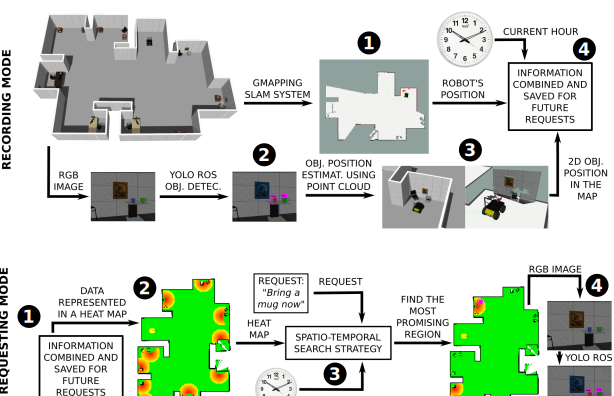
\includegraphics[width=1\textwidth]{figs/system_overview.png}
    \caption[Flowchart that explains how our LSOS system works.]{Flowchart that explains how our LSOS system works. The top half is the mode in which the robot gathers information about the environment, and the bottom half is the one that is executed when the robot is active with finding an object.}
    \label{fig:system_overview}
\end{figure}

The first mode, recording, is responsible for gathering and saving all the data that our LSOS system needs, as the upper half of Figure~\ref{fig:system_overview} illustrates. The goal of this mode is to fulfill our OS system's requirements, as mentioned earlier. The more data it gathers from the environment, the more efficient our OS system becomes. In summary, the recording mode relies on an object-detection algorithm and a SLAM system. We use YOLO for object-detection (see Chapter~\ref{chap:2_you_only_look_once}), as it is a robust and popular package for such task, and apply the Gmapping package, a laser-based SLAM for building a 2D grid map~\cite{Bjelonic2018Yolo, Gerkey2020Gmapping}. 
During the execution of this mode, when an object is within the camera's point of view, YOLO detects it.  A depth camera with a point cloud measures the distance between the robot and the object, and then our system calculates its position in the map given the robot's pose. Once the robot's and object's position are known, our system saves this information, along with the detection hour and the class of the object provided by YOLO. This recording mode can be executed hourly, daily, or while the robot performs any other task. It is also important to highlight that our OS system is not restricted to YOLO and Gmapping. Any object-detection and SLAM package, respectively, provide the same data type our system saves, and hence, could be used in our system. 

The second mode, requesting, is performed by our LSOS system when the robot is active with finding an object, i.e., when someone requests it to look for a target object. It worth to mention that when when our system is requested to search for a target object, it does not differentiate the instances of that object. For example, when searching for a book, both \textit{The Lord of the Rings} and \textit{Don Quixote} (and any other book) are valid options to LSOS. Hence, the target object represents a class of objects, and finding any instance that belongs to that class is sufficient. Furthermore, this mode aims to find the target with the robot traveling the shortest distance to save time and the robot's resources. All the data gathered in the recording mode plays an important role here, as it helps to improve the estimations of our LSOS system. The more data the recording mode records, the better is the estimation computed by the requesting mode. The lower half of Figure~\ref{fig:system_overview} illustrates the entire requesting process. The requesting mode builds a heat map out of the recorded data to estimate which environment regions are more promising to locate the target object in. In contrast to many OS systems in the literature, our proposal considers the hour that objects have been detected and compares them with the request hour. Therefore, when the robot receives a request, it goes to the warmest spot in the heat map, i.e., region of the environment where is more liley to find the target object. Lastly, if the requesting mode is executed before the recording one, and no data from the environment is available, our OS system would perform a brute force search since no information is available to improve its performance.

Although our LSOS system makes predictions based on the arrangement (organisation) of objects, it does not have a separate training phase to learn the objects' presence, like machine learning algorithms.
In fact, both modes (recording and requesting) can run in parallel, albeit the more information the map contains prior to the search, the better the search results tend to be. Another important point is that the semantic map in which the searches are based is not a black box. On the contrary, it relies on a probabilistic approach that infers the most promising regions to find the target object by recording how people interact with it. Besides, as the experiments presented below suggest, a small amount of data is enough for our system to succeed.

\section{Our LSOS system's search strategy}
\label{sec:semantic_strategy} 
This section details our OS system and how it works. It starts with the description of the heat map module in Sections~\ref{subsec:heat_map} and ~\ref{subsec:inverting_kernel}, with explanation of how our LSOS system builds it based on the gathered data in the recording mode. Finally, Section~\ref{subsec:final_formula} presents the goal computation, which explains how our OS system estimates the most promising map regions to find the target object, i.e., the warmest spots in the heat map. It also discuss how our OS system behaves when the object is not found at the most promising region of the map.

%\subsection{Custom object detection model}
%\label{subsec:custom_obj_detect_model} 
%TO DO by Farzan

\subsection{The Heat Map and the representation of the objects' presence}
\label{subsec:heat_map}
The heat map is a visual technique widely used for visualizing complex spatial patterns, proposed by Kinney~\cite{Kinney1993Heatmaps}. It provides a meaningful and straightforward understanding for humans and processing programs. In this chapter, the discrete distribution of objects' presence is processed into a continuous color distribution, in which the most likely regions to find the target object are intuitively revealed. 

The 2D grid map $\bs{m}$ that has been built by the SLAM system during the recording mode is used for computing the heat map~$\bs{h}$. Both maps are equal in terms of the number of cells and size, but the difference is that a cell $\bs{m}_i \in \bs{m}$ is either free, occupied, or unknown, whereas the same cell $\bs{h}_i \in \bs{h}$ is the heat value that represents how likely that location is to contain a certain object. A cell in both $\bs{m}$ and~$\bs{h}$ represents exactly the same place in the environment. Hence, only the cells that are either free or occupied in $\bs{m}$ are likely to have a heat value different than zero in $\bs{h}$, as there are no objects on unknown regions in~$\bs{m}$.

All the~\textit{n} objects that have been detected in the recording mode are represented by the set $\mathbf{O}$, in which $\mathbf{O} = \{\bs{o}_1, \bs{o}_1, \cdots, \bs{o}_n\}$. Each $\bs{o}_j \in \mathbf{O}$ is composed by its position within~$\bs{h}$, its class, the hour it has been detected, and the robot's position during the detection, i.e., $\bs{o}_j = (\bs{o}_j^p, \bs{o}_j^c, \bs{o}_j^h, \bs{o}_j^r)$, respectively. To compute~$\bs{h}$, we represent the presence of the object $\bs{o}_j \in \mathbf{O}$ by a weighted circular kernel $K(\cdot)$ of radius~\textit{r}. Let~\textbf{T} be the set of cells within the area of $K(\cdot)$ for a given~\textit{r}, and $\mathbf{T} \in \bs{h}$. For all cells $\bs{h}_i \in \mathbf{T}$, $K(\cdot)$ is defined as
\begin{equation}
K\big(D(\bs{h}_i,\bs{o}_j^p), \bs{o}_j^h\big) = 
  \begin{cases}
 W(rh, \bs{o}_j^h)Q(\bs{h}_i)(1 - \frac{d}{r}), & \quad  $if$~d \leqslant~r\\ 
 \hfill 0,  & \quad~$otherwise$
  \end{cases}    
\label{eq:kernel_definition}
\end{equation}
where~$D(\bs{h}_i,\bs{o}_j^p)$ is the Manhattan distance from the current cell being measured, $\bs{h}_i \in \mathbf{T}$ to the centre of the kernel, $\bs{o}_j^p \in \bs{h}$. The function $Q(\cdot)$ is defined as
\begin{equation}
Q(\bs{m}_i) = 
  \begin{cases}
    0, & \quad \text{if}~\bs{m}_i~\text{is unknown in }\bs{m}\\ 
    1, & \quad \text{otherwise}
  \end{cases} 
\label{eq:q_function_unknown_cells}  
\end{equation}
and it checks whether a cell $\bs{m}_i$ is unknown in $\bs{m}$. The other function $W(rh, \bs{o}_j^h)$ computes the difference between the hour the object has been detected, $\bs{o}_j^h$, and the hour the robot is requested to perform the search, $rh$. This difference is then used to compute the weight factor of the object $\bs{o}_j$, since the smaller is the hour difference, the more important that object becomes to the search. This function is defined as
\begin{equation}
W(rh, \bs{o}_j^h) = 1 - \frac{\left | rh - \bs{o}_j^h \right |}{12} 
\label{eq:hour_weight}
\end{equation}
Here is important to mention that we use the 24-hour notation. Hence, $W(rh, \bs{o}_j^h)$ is equal to one when $rh$ and $\bs{o}_j^h$ are equal, and it is zero when they are 12 hours apart from each other, i.e., the largest difference in hours between two different time stamps. 
%In this chapter, Equation~\ref{eq:hour_weight} computes the weight of the object $\bs{o}_j$, in which the closer both hours are, the more important the object becomes for the search. 
For example, if ou LSOS system detected an object two times, at 8:00 in position A and 14:00 in position B, and it is performing the search at 10:00, it will probably start searching the object in A, as 8:00 is closer to 10:00 than 14:00.

The first part of computing the heat map~$\bs{h}$ is depicted in Figure~\ref{fig:kernel_heat_map}. 
%The map of the environment in simulation is illustrated in Figure~\ref{fig:kernel_heat_map}-(a), and in Figure~\ref{fig:kernel_heat_map}-(b) the map~\textbf{M} is presented. 
The outcome of Equation~\ref{eq:kernel_definition} is shown in Figure~\ref{fig:kernel_heat_map}c, in which every object from~\textbf{O} is represented by the kernel $K(\cdot)$. It is important to notice that the warmest cells in~$\bs{h}$, Figure~\ref{fig:kernel_heat_map}c, are at the objects' positions in Figure~\ref{fig:kernel_heat_map}a. 

\begin{figure}[!h]
\centering
\includegraphics[width=.8\textwidth]{figs/environment_2Dgrid_heatmap_kernel.png}\\
(a)\hspace{2.8 cm}(b)\hspace{2.8cm}(c)
\caption[Example of the computed heat map given a set of detected objects.]{Example of the computed heat map given a set of detected objects. (a) is the simulated environment with 10 objects spread in seven rooms. (b) is the 2D grid map built by Gmapping. (c) is the heap map built by our OS system, considering the map in (b) and the detected objects in (a). The warmer regions represent their position within the map.}
\label{fig:kernel_heat_map}
\end{figure}

The computed heat map $\bs{h}$ in Figure~\ref{fig:kernel_heat_map}c indicates which regions our LSOS system should search, since it does not consider the colder spots (green region) in~$\bs{h}$. Besides, the class of an object helps to focus the searching in more promising regions, as there is no point in searching in a warm spot where there is only a book if our system is looking for a mug. Since the class of a detected object $\bs{o}_j$ is known, $\bs{o}_j^c$, our system ignores warm spots from objects with different classes than the target one.

A third adjustment in the process of computing the heat map comes with a subtraction on the circular kernel's angle. During the search, our OS system guides the robot towards the edge of the most promising kernel. The edge, yellow cells  in~$\bs{h}$, is one of the best regions to place the robot because it is the ideal distance between the robot and the kernel center (or the object's position). However, despite the ideal distance, positioning the robot at any place over the edge of the kernel does not ensure the object will be either recognised or even within the camera's field of view. This issue is illustrated in Figure~\ref{fig:bad_robot_placement}, in which the robot is quite close to the compute monitor at the edge of its kernel, but yet the object detection module is not able to detect it. Alternatively, the most appropriate position to place the robot would be the same one that the robot has been in when recognizing the object during the recording mode. Thus, it is most likely that the object detection module will recognize the object once again if the robot assumes a similar pose it has assumed before. Hence, our heat map~$\bs{h}$ is built considering the kernel $K(\cdot)$ in Equation~\ref{eq:kernel_definition} with an acute angle, instead of considering a \ang{360} one. For a given object~$\bs{o}_j$, its kernel's angle is defined considering its robot's position when it has been recognised, i.e., $\bs{o}_j^r$. Figure~\ref{fig:good_robot_placement} illustrates the advantage of restricting the kernel's angle, in which the object detection module recognize the computer monitor.

\begin{figure}[!h]
\centering
\includegraphics[width=.6\textwidth]{figs/bad_robot_placement_1.png}\\ 
(a)\hspace{3.5cm}(b)
\\
\includegraphics[width=.6\textwidth]{figs/bad_robot_placement_2.png}
\\(c)\hspace{3.5cm}(d)
\caption[Example of the robot at the edge of the kernel, and yet not recognising the object.]{Example of the robot at the edge of the kernel, and yet not recognising the object. (a) is the environment in simulation, (b) is the robot in $\bs{m}$, (c) is the robot in~$\bs{h}$, and (d) the current image capture by the robot's camera. %Even though the robot is considerably close to the computer monitor, the object detection module can not detect it due to the point of view.
}
\label{fig:bad_robot_placement}
\end{figure}

\begin{figure}[!h]
\centering
\includegraphics[width=.6\textwidth]{figs/good_robot_placement_1.png}\\
(a)\hspace{3.5cm}(b)
\\
\includegraphics[width=.6\textwidth]{figs/good_robot_placement_2.png}
\\(c)\hspace{3.5cm}(d)
\caption[Example of the modified kernel with an acute angle, and the recognised object.]{Example of the modified kernel with an acute angle, and the recognised object. (a) is the environment in simulation, (b) is the robot in $\bs{m}$, (c) is the robot in~$\bs{h}$, and (d) the current image capture by the robot's camera. %It is possible to note that the robot's current position is suitable for recognizing the object since it is similar to the one the robot had assumed before when the object was recognised for the first time.
}
\label{fig:good_robot_placement}
\end{figure}

The adjustments performed while computing the heat map~$\bs{h}$ plays an important role in our LSOS system. Figure~\ref{fig:step_by_step_search_space_reduction} represents the step by step of each adjustment, and the outcome is a few warmer spots in~$\bs{h}$. Besides saving computational resources by reducing the amount of regions to search, there is also an increase in the chances of detecting the target object by the proper robot positioning. 

\begin{figure}[!h]
\centering
\includegraphics[width=.9\textwidth]{figs/step_by_step.png}\\
(a)\hspace{3cm}(b)\hspace{3cm}(c)\hspace{3cm}(d)
\caption[Step by step of the space reduction performed by our OS system.]{Step by step of the space reduction performed by our OS system. (a) is the empty~$\bs{h}$, (b) is the representation of all objects from~\textbf{O} with the circular kernel $K(\cdot)$, (c) is the kernels' angle reduction given the robot's position of each object, and (d) is the outcome of considering only objects with the same class as the target's one and the other ones are ignored.}
\label{fig:step_by_step_search_space_reduction}
\end{figure}

\subsection{Inverted kernel $IK(\cdot)$}
\label{subsec:inverting_kernel}
Our system performs another operation to make it easier to find the target object. In OS systems, one of the main goals is to place the robot at the most appropriate place to accomplish the task. In this chapter, as we already mentioned, the most promising regions to place the robot are at the kernels' edges due to the ideal distance to the objects. However, such edges in the kernel $K(\cdot)$ presented in Equation~\ref{eq:kernel_definition} are the coldest regions within the kernel area, as the warmest one is at the kernel's center. Hence, if our system computes the inverse $IK(\cdot)$, the warmest regions becomes the ones at the edge, i.e., the ideal spots to place the robot during the search are the ones with the highest heat value. The $IK(\cdot)$ is similar to the one presented in Equation~\ref{eq:kernel_definition}, and it is defined as

\begin{equation}
IK\big(D(\bs{h}_i,\bs{o}_j^p), \bs{o}_j^h\big) = 
  \begin{cases}
 W(rh, \bs{o}_j^h)Q(\bs{h}_i)\frac{d}{r}, & \quad  if d \leqslant~r\\ 
 \hfill 0,  & \quad \text{otherwise}
  \end{cases}    
\label{eq:inverse_kernel} 
\end{equation}

In summary, the difference between Equations~\ref{eq:kernel_definition} and~\ref{eq:inverse_kernel} is that the former computes~$\bs{h}$ as the warmer regions being the object's position, whereas the latter computes~$\bs{h}$ as the warmer regions being the ideal place to position the robot during the search. Figure~\ref{fig:different_kernel_comparison} shows their difference. 

%\begin{figure}[!h]
%\centering
%\hspace{.4cm}(a)\hspace{2.6cm}(b)\\
 %\rotatebox{90}{\hspace{1cm}\text{Circular kernel}}
 %\includegraphics[width=.5\textwidth]{figs/normal_inverse_kernels_complete.png}\\
 %\rotatebox{90}{\hspace{1cm}\text{Reduced kernel}}
 %\includegraphics[width=.5\textwidth]{figs/normal_inverse_kernels_reduced_angle.png}
%\caption{The difference between the kernel and its inverse. (a) is the kernel presented in Equation~\ref{eq:kernel_definition}, in which its center is the warmest spot. (b) is the inverse kernel, defined by Equation~\ref{eq:inverse_kernel}, in which the inverse kernel's edge are the warmest spots. (a) intuitively represents the object's presence, whereas (b) represents the best places to position the robot to find a target object.}
%\label{fig:different_kernel_comparison}
%\end{figure}

\begin{figure}[!h]
\centering
  Normal kernel\hspace{4.5cm}Inversed kernel\\
  \vspace{.3cm}
 \includegraphics[width=.45\textwidth]{figs/normal_kernel_complete_reduced.png}
 \includegraphics[width=.45\textwidth]{figs/inversed_kernel_complete_reduced.png}\\
 (a)\hspace{3cm}(b)\hspace{3cm}(c)\hspace{3cm}(d)

\caption[The difference between the normal kernel and its inverse.]{The difference between the normal kernel and its inverse. (a) and (b) represent the normal kernel, the circular and reduced version, respectively. (c) and (d) represent the same for the inversed version of the same kernel.}
\label{fig:different_kernel_comparison}
\end{figure}

Despite the easy readability by humans of~$\bs{h}$ built by Equation~\ref{eq:kernel_definition}, due to the intuitive object's presence representation, for our OS system Equation~\ref{eq:inverse_kernel} provides the most appropriate~$\bs{h}$. Therefore, for now on, all references of~$\bs{h}$ within this work considers that it has been built using Equation~\ref{eq:inverse_kernel}.

\subsection{Goal computation in the request mode}
\label{subsec:final_formula}

The process of building the heat map~$\bs{h}$ and reducing the search space is the first part of our OS system, in which we represent the data from the recording mode in~$\bs{h}$. In addition to that, it is also necessary to compute the goal, i.e., the most promising spot in~$\bs{h}$ that our system estimated to the robot go and find the target object. This computation is performed when the robot is requested to look for the target object.%In Figure~\ref{fig:step_by_step_search_space_reduction}-(d), for example, the goal would be one of the two remaining warm spots since they represent objects with the category than the target one. 

The goal computation is similar to the heat map construction because we also use a kernel approach. Our idea here is to analyse the whole~$\bs{h}$ in several circular kernels, and get the cell $\bs{h}_i^*$ that neighbours have the highest probability of containing the target object, $\bs{o}_j$, for the request hour, $rh$. The final equation for computing the goal cell $\bs{h}_i^* \in \bs{h}$ is defined as
\begin{equation} 
\bs{h}_i^* = \underset{\bs{h}_i\in\bs{h}}{\text{arg max}}\big(\varphi(\bs{h}_i, \bs{o}_j, rh)\big)    
\label{eq:final_equation}
\end{equation}
in which the function $\varphi(\bs{h}_k)$ computes the possibility of the cell $\bs{h}_i$ contains the target object, $\bs{o}_j$. It is defined as
\begin{equation}
\varphi(\bs{h}_k,\bs{o}_j, rh) = \sum_{\bs{h}_i}^{\mathbf{T}}H(\bs{h}_i,\bs{o}_j, rh)
\label{eq:psi_function}
\end{equation}
where $\mathbf{T}$ is a set of cells within the kernel area and $\mathbf{T} \subset \bs{h}$ centred in $\bs{h}_k$. The function $H(\cdot, \cdot, \cdot)$ returns the heat value (or probability) of the target object $\bs{o}_j$ being in the cell $\bs{h}_i$, at the request hour, $rh$.


%and $K'(\cdot)$ is a simpler version of the kernel presented in Equation~\ref{eq:kernel_definition} defined as
%\begin{equation}
%K'(d) = 
%  \begin{cases}
% a, & \quad  \text{if~}d\leqslant r\\ 
% \hfill 0,  & \quad \text{otherwise}
%  \end{cases} 
%\label{eq:kernel_goal}
%\end{equation}
%$r$ is the radius of $K'(\cdot)$, different from the one used in Equation~\ref{eq:kernel_definition}, and~\textit{d} is the Manhattan distance. 

It is possible that for a certain request to our OS system, there are multiple regions in~$\bs{h}$ that register the presence of instances of the target object. Thus, our OS system computes Equation~\ref{eq:final_equation} over~$\bs{h}$ and sorts the multiple $\bs{h}_i^*$ according their likelihood. The robot is moved towards the most likely one, and if the target object at that position is not found, the robot proceeds to the second most promising $\bs{h}_i^*$. This process is repeated until the robot visits all regions that register the presence of the target object. Lastly, in the worst case where the object was not found in any promising regions, the robot inspects all unvisited rooms, similar to a brute force search.

\section{Experiments and Results} 
\label{sec:chap2_experiments_results}
This section is divided into four subsections. %Section~\ref{subsec:object_detection_module} presents the experiment with Yolo, comparing our customized model with the standard ones publicly available. 
Section~\ref{subsec:datasets_simulation} discusses the dataset and simulation setup used throughout the experiments. Section~\ref{subsec:comparison_approaches} explains the other two OS systems that we compare against our proposal, followed by Section~\ref{subsec:simulated_experiment_setup} that presents the experimental setup to which the three OS systems have been tested, along with their respective performances. Section~\ref{subsec:hh106_dataset} shows the performance of our LSOS system in estimating the person's presence given the HH106 dataset.

%\subsection{Object detection module}
%\label{subsec:object_detection_module}
%The Yolo object detection system can be either used with a pre-trained model, in which the Yolov2 and Yolov3 are the most popular models, or with a new customized one. This experiment aims to measure the Yolov2, Yolov2-tiny, and Yolov3's efficiency against our customized one, in detecting objects in the simulation. We have created the scenario illustrated by Figure~\ref{fig:darknet_experiment}, in which the robot follows the red path, autonomously visiting all the three objects, computer monitor, book, and mug. The robot remains still in front of each object for seven seconds, and then it continues to the next one. We collect the data about each model's performance only within these seven seconds.
%
%The performance of each model was measured by its FPS rate, object prediction accuracy, and recall. The experiment was repeated five times for each model, with the robot starting at the same position in every run, and Table~\ref{tab:darknet_experiment} presents the results. As each model was repeated five times, we calculated the recall of each model while detecting every object, along with the average of the detection belief from the correct detections. If a model failed to recognize the object in a run, we considered the prediction accuracy for that object as zero.
%
%\begin{figure}[!h]
%\centering
%\includegraphics[width=.7\textwidth]{figs/darknet_experiment_edited.png}
%\caption[The setup in simulation for the experiments with different models for Yolo.]{The setup in simulation for the experiments with different models for Yolo.}
%\label{fig:darknet_experiment}
%\end{figure}
%
%\begin{table*}
%\centering
%\caption[Performance of each tested model tested in our experiment with Yolo.]{Performance of each tested model tested in our experiment with Yolo.}
%\begin{tabular}{cc|ccc}\toprule
%\multicolumn{2}{c|}{\textbf{Yolo's models}} & \multicolumn{3}{c}{\textbf{Objects}}\\
%\textbf{Name} & \textbf{Data} & \textbf{Comp. Monitor} & \textbf{Book}    & \textbf{Mug}  \\\midrule
%\multirow{3}{*}{YoloV2-tiny} & Acc. Aver. & 46.0~$\pm$~0 & 45.50~$\pm$~7.78 & 64.20~$\pm$~8.70
%\\
% & Recall & 20\% & 40\% & 100\%\\
% & FPS & 12$\sim$160 & 12$\sim$160 & 12$\sim$160
%\\\midrule
%\multirow{3}{*}{YoloV2} & Acc. Aver. & 37.00~$\pm$~21.73 & 62.00~$\pm$~8.28 & 72.80~$\pm$~12.28
%\\
% & Recall & 40\% & 100\% & 100\%\\
% & FPS & 40$\sim$70 & 40$\sim$70 & 40$\sim$70
%\\\midrule
%\multirow{3}{*}{YoloV3} & Acc. Aver. & 47.00~$\pm$~0 & 63.00~$\pm$~22.58 & 68.00~$\pm$~29.56
%\\
% & Recall & 20\% & 80\% & 100\%\\
% & FPS & 20$\sim$35 & 20$\sim$35 & 20$\sim$35
%\\\midrule
%\multirow{3}{*}{Ours} & Acc. Aver. & 91.60~$\pm$~9.13 & 87.00~$\pm$~9.70 & 75.20~$\pm$~24.87
%\\
%& Recall & 100\% & 100\% & 100\%\\
% & FPS & 12$\sim$16 & 12$\sim$16 & 12$\sim$16
%\\\bottomrule
%\end{tabular} 
%\label{tab:darknet_experiment}
%\end{table*}
%
%In general, our custom model presented the best tradeoff between accuracy and FPD rate. Besides, it was the only one that recognised the three objects in all five runs, which is shown by its maximum recall in all three objects. For the other three models, while the robot was still and heading at the objects, they did not recognize the objects in all runs, mainly the computer monitor. This failure in detecting is observed by the low recall for the other models. It is worth mentioning that even though the other three models failed in detecting the objects, they never misrecognised an object. Our model recognised the computer monitor in all five runs, and its belief was 91.60\% on average. Even though the Yolov2-tiny has the highest FPS rate, 12$\pm$160, it recognised the computer monitor just once in the five runs and did not perform well in general. Although the FPS rate of our custom model is the lowest one, it does not compromise the general performance of our OS system. Besides, we believe it is a fair tradeoff given its success in detecting the objects with high accuracy. 


\subsection{Simulation and dataset}
\label{subsec:datasets_simulation} 
Our proposal is to let the robot autonomously navigate through the environment until the target object's position. Such autonomy demands motion freedom that exists either in the real world or in a simulated environment that allows the robot to make decisions about its movement freely. Besides, as most of the OS systems in the literature are proposed assuming static environments, ignoring changes in the objects' position, the majority of the publicly available datasets are recorded in static environments. Unlike them, our LSOS system considers the semantic information of objects' position changes, and also uses other specific sorts of data, like the robot's pose. We assume that the environment is not static all the time. Hence, for testing and evaluating our system, we need a long-term dataset that provides information about the history of the objects' position, i.e., their location over time and what time they have been recognised at a specific location.

To the best of our knowledge, no dataset in the literature accomplishes our requirements, with all the high-level information our proposal needs. The datasets consist of a robot either moving through an environment many times but without objects' information or a single run and the class of the recognised object~\cite{Howard2003Radish, Luo2007Incremental, Afif2019ANovel}. Besides, even though we could annotate the objects' position over time by watching the video from the robot's camera, we would not be able to move the objects as we want to mimic different patterns and routines, and we can not ensure our annotations would be correct. 

Therefore, we have used the Gazebo simulator to create an environment similar to an office with many small rooms connected, illustrated in Figure~\ref{fig:simulated_environment}a. It measures 20.5m by 14.5m and contains seven rooms and objects in ten different places. We have chosen objects easily found in most offices, such as books, mugs, computers, and smartphones. Instances of different object classes are found in our simulated environment, at least in two different places, to test our system in scenarios with multiple promising places simultaneously. Creating our environment allows us to change the object's position and even remove some of them. Thus, we can record the data using the recording mode with the objects' presence in different patterns, simulating multiple human routines. For this experiment, we use the Husky robot from Clearpath, Figure~\ref{fig:simulated_environment}b. It is an unmanned ground vehicle equipped with a 2D lidar laser and an Intel RealSense depth camera.

Despite the lack of public datasets appropriate for our LSOS system, we still would like to evaluate our OS system in a real scenario. Therefore, we used a long-term dataset where the target object is a human. The HH106 provides continuous ambient sensor data for human activity recognition, collected by 37 sensors spread over a nine-room apartment for two months~\cite{Cook2010Learning}. A single volunteer occupies the apartment, generating over 259.900 instances of data within the two months. We have considered only the motion sensors for our experiments, as they indicate where the volunteer is at a specific time. Figure~\ref{fig:hh106_dataset} shows the apartment's floorplan and where the sensors have been placed for recording the data.


\begin{figure}[!h]
\centering

\includegraphics[width=.42\textwidth]{figs/simulated_environment.png}
\includegraphics[width=.25\textwidth]{figs/husky_robot.png}\\
\hspace{1cm}(a)\hspace{5cm}(b)
\caption[The seven-rooms environment created on Gazebo simulator and the Husky robot.]{(a) is the seven-rooms environment created on Gazebo simulator, and (b) is the Husky robot used throughout the experiments presented in this chapter.}
\label{fig:simulated_environment}
\end{figure}

\begin{figure}[!h]
\centering
\includegraphics[width=.75\textwidth]{figs/hh106sensor_map.png}
\caption[The floorplan of the single-resident apartment from the HH106 dataset.]{The floorplan of the single-resident apartment from the HH106 dataset.}
\label{fig:hh106_dataset}
\end{figure}

\subsection{Two other object search systems to be compared against ours}
\label{subsec:comparison_approaches}
We compare our LSOS system with a Brute Force and a Last Seen OS systems. They are briefly presented below as well as why they have been chosen to be tested in this chapter.

\subsubsection{Brute Force OS system}
\label{subsubsec:brute_force_os}
Inspired by security patrol robots that repeat the same route from time to time, this system makes the robot visit all locations according to a predefined route. Besides the robot's route, no information about the environment or the objects' presence is provided beforehand. In the field of OS, it is known as a brute force approach, which explains its name. Figure~\ref{fig:brute_force_os} depicts the clockwise route periodically repeated by the robot. Like any other brute force-based OS system, it does not ensure the robot will achieve the optimal performance in terms of the use of resources (battery and time), even though the robot finds the target object in most cases. In this chapter, such a system is the benchmark to be considered.

\begin{figure}[!h]
\centering
\includegraphics[width=.6\textwidth]{figs/brute_force_route2.png}
\caption[The robot's route for the Brute Force OS system.]{The robot's route for the Brute Force OS system. The squared R is the robot's initial position, and then it follows the clockwise track in red from location A until location J, finishing back in R.}
\label{fig:brute_force_os}
\end{figure}

\subsubsection{Last Seen OS system}
\label{subsubsec:last_seen_os}
This system is similar to our proposal in terms of the usage the semantic information about the organisation of objects over time. It guides the robot to the map spot where it has detected an instance of an object class that is equal to the target object, but only the most recent object detection. The difference to our proposal is that it only considers the most recent observation, neglecting the rest of the objects' historic positions. Even though this system may save time and the robot's resources by guiding the robot straight to a specific spot, it does not ensure that the object will be found. The lack of information from the past may mislead the system, reducing its efficiency.

\subsection{Simulated Experiment Setup}
\label{subsec:simulated_experiment_setup}

The three OS systems have been tested in different scenarios in simulation, with five objects' position patterns. Throughout the tests, we considered a simulated environment with objects being positioned in ten different locations, as can be seen in Figure~\ref{fig:brute_force_os}. The systems have to find any instance of the target object, which is a mug. These instances could be in location A or H, Figure~\ref{fig:brute_force_os}. We have chosen these locations because they are on opposite directions of the robot's initial position R in Figure~\ref{fig:brute_force_os}. Hence, it highlights the efficiency of an OS system. If an OS system does not make the right decision since the begining of the search, its performance will be inefficient.

The Table~\ref{tab:objects_presence_setups} depicts the data that is used in the experiments. To get the data, a robot repeated ten times a routine of visiting all rooms of our simulated environment while running the recording mode. Starting at 3:00, every routine was performed two hours apart, except for the period between 11:00 and 15:00. When an instance of mug was detected, our system recorded where it was (location A or H), and the hour of the detection. We could position instances of mug in many possible arrangements in the simulation, but this section does not intended to test all of them. Instead, we defined five different arrangements (patterns) for the objects, namely \textit{Static}, \textit{Static-Inv}, \textit{Mobile}, \textit{Mobile-Inv}, \textit{Shift}. The five patterns in Table~\ref{tab:objects_presence_setups} have been manually designed as if the robot had recorded them on different days, and they are not related to each other. The experiments in this section aim to compare the three OS systems in different scenarios and investigate our OS system's performance in searches with little data available about the object's position. Hence, when we test our OS system based on \textit{Mobile}, for example, there are only its ten moments of the day that mugs have been detected to be considered for the estimations. 
\begin{table*}[!h]
\centering
\caption[Mug's position recorded in five setups by the recording mode of our proposal.]{Mug's position recorded in five setups by the recording mode of our LSOS system.}
\begin{tabular}{c|ccccc|ccccc}\hline
\multirow{3}{*}{Pattern}                                         & \multicolumn{10}{c}{Recording hours}\\

                                         & \multicolumn{5}{c}{Morning} & \multicolumn{5}{c}{Evening}\\
\cmidrule(rl){2-6} \cmidrule(rl){7-11}                                         
  & 3:00 & 5:00 & 7:00 & 9:00 & 11:00 & 15:00 & 17:00 & 19:00 & 21:00 & 23:00  \\\hline
\textit{Static} & A & A & A & A & A~ & ~H & H & H & H & H
\\\hline
\textit{Static-Inv} & H & H & H & H & H~ & ~A & A & A & A & A
\\\hline
\textit{Mobile} & A & H & A & H & A~ & ~H & A & H & A & H
\\\hline
\textit{Mobile-Inv} & H & A & H & A & H~ & ~A & H & A & H & A
\\\hline
\textit{Shift} & H & H & H & H & A~ & ~A & A & A & A & H
%\\\midrule
%6 & H & H & H & H & A~ & ~A & A & A & A & H
\\\hline
\end{tabular}
\label{tab:objects_presence_setups}
\end{table*}

An instance of a mug has been detected both in locations A and H at different hours.  On \textit{Static}, the mug was in location A during the morning, from 3:00 until 11:00, and in location H during the evening, from 15:00 until 23:00. The opposite happened on \textit{Static-Inv}, in which the mug was also moved between 11:00 and 15:00. On \textit{Mobile} and \textit{Mobile-Inv}, it is possible to note that the mug was moved more often, illustrating a different pattern of \textit{Static} and \textit{Static-Inv}. On \textit{Shift}, the \textit{Static-Inv} patter is shifted back by one hour, and the mug is in a different location on the last hour of each period of the day (morning and afternoon). %Setup 6 is the combination of all previous setups, and it is proposed to test our OS system under a more significant amount of data gathered for the searching.

For every setup in Table~\ref{tab:objects_presence_setups}, the three OS systems were tasked with finding an instance of a mug at noon and midnight. These two requesting hours have been chosen because they are not within Table~\ref{tab:objects_presence_setups}. Hence, the tested OS systems are not aware of the mug's position at these times. The Table~\ref{tab:ground_truth_mugs} shows the mug's location for each requesting hour, and it is used as ground-truth for our experiments. We considered the mug remained at the position it was when detected the last time within each period of the day, i.e., at 11:00 and 23:00. Hence, the values of Table~\ref{tab:ground_truth_mugs} are equal to the columns 11 and 23 of Table~\ref{tab:objects_presence_setups}. It is important to highlight that the information in Table~\ref{tab:ground_truth_mugs} is only used to compute the results, and this data is not provided to any of the OS systems tested. 

The Brute Force system repeated its route in every test, whereas the Last Seen considered the latest detection hour of every setup, which is at 23:00 for the five setups. Our proposed semantic OS system used all the data from each setup, e.g., for a search in \textit{Static}, it uses only the data from its ten detections. The robot's traveled distance measures the system's performance, i.e., the length of the robot's trajectory until either finding an instance of the target object or reporting that the object has not been found. Therefore, the shorter the traveled distance, the better is the system's performance.
 
\begin{table*}[!h]
\centering
\caption[Ground-truth of the mug's position for every setup according to the requesting hours.]{Ground-truth of the mug's position for every setup according to the requesting hours.}
\begin{tabular}{c|c|c}\hline
\multirow{2}{*}{Setups}                                           & \multicolumn{2}{c}{Requesting hours}\\
     & ~~~12:00           & 00:00  \\\hline
\textit{Static} & ~~~A & H
\\\hline
\textit{Static-Inv} & ~~~H & A
\\\hline
\textit{Mobile} & ~~~A & H
\\\hline
\textit{Mobile-Inv} & ~~~H & A
\\\hline
\textit{Shift} & ~~~A & H
\\\hline
\end{tabular}
\label{tab:ground_truth_mugs}
\end{table*}

\subsection{Results and discussion from the simulated experiments}
\label{subsec:results_discussion}
An OS system should efficiently find the target object, saving as much time and robot's battery as possible. This section presents and discusses the results of the three OS systems tested in this chapter. We measured their performance by computing the robot's traveled distance for searching the target object and whether they managed to find it. Every combination of OS system, requesting hour, and setup was tested ten times, and from these tests, we computed the average and the standard deviation of the traveled distances, which are shown in Figure~\ref{fig:all_results_setups}.% Figs.~\ref{fig:day_one}~\ref{fig:day_two}~\ref{fig:day_three}~\ref{fig:day_four}

The \textit{Static} and \textit{Static-Inv} are characterized by only one change in the mug's position throughout the day, which happened at some time between 11:00 and 15:00. Their difference is that one is the inverted version of the other. In the results from both setups, Figures~\ref{fig:static_setup} and ~\ref{fig:static_inv_setup}, respectively, when the Last Seen OS system had to find an instance of mug at noon, it was the only one that failed. That is due to the mug's position at 23:00 in both setups. Their last mug detection in Table~\ref{tab:objects_presence_setups} happened at 23:00 in location H for the \textit{Static}, and in location A for the \textit{Stativ-Inv}. Hence, the Last Seen system wrongly guided the robot towards the opposite location in each setup. The Brute Force and our system found an instance of mug in both request searches for the two setups. However, there is a considerable difference in their performances for the request search at midnight in the \textit{Static}, Figure~\ref{fig:static_setup}, and for the one at noon in the \textit{Stativ-Inv}, Figure~\ref{fig:static_inv_setup}. In such requests and setups, the mug was in the location H, as shown in Table~\ref{tab:ground_truth_mugs}, and the Brute Force system makes the robot travel a longer distance until it finds an instance of mug, as illustrated by the robot's trajectory in Figure~\ref{fig:BF_roomH2}. In contrast, the Last Seen and our systems achieved the same goal traveling a distance three times shorter, like the examples in Figures~\ref{fig:LS_roomH2} and \ref{fig:OUR_roomH2}, respectively. For the request search at noon in the \textit{Static}, and at midnight for the \textit{Static-Inv}, the three systems have a similar result because the mug is in location A, Table~\ref{tab:ground_truth_mugs}, which is the first location the Brute Force guides the robot to, as shown in Figure~\ref{fig:BF_roomA2}. Therefore, despite not reasoning over the available data, the Brute Force presents a similar result as ours.

\begin{figure*}[t]
     \centering
      \begin{subfigure}[b]{0.48\columnwidth}
         \centering
         \includegraphics[width=1.1\textwidth]{figs/static_setup.png}
         \caption{\textit{Static} setup}
          \label{fig:static_setup}
     \end{subfigure}
      \begin{subfigure}[b]{0.48\columnwidth}
         \centering
         \includegraphics[width=1.1\textwidth]{figs/static_inv_setup.png}
         \caption{\textit{Static-Inv} setup}
         \label{fig:static_inv_setup}
     \end{subfigure}\\[.5em]
      \begin{subfigure}[b]{0.48\columnwidth}
         \centering
         \includegraphics[width=1.1\textwidth]{figs/mobile_setup.png}
         \caption{\textit{Mobile} setup}
         \label{fig:mobile_setup}
     \end{subfigure}
      \begin{subfigure}[b]{0.48\columnwidth}
         \centering
         \includegraphics[width=1.1\textwidth]{figs/mobile_inv_setup.png}
         \caption{\textit{Mobile-Inv} setup}
         \label{fig:mobile_inv_setup}
     \end{subfigure}\\[.5em] 
      \begin{subfigure}[b]{0.48\columnwidth}
         \centering
         \includegraphics[width=1.1\textwidth]{figs/shift_setup.png}
         \caption{\textit{Shift} setup}
         \label{fig:shift_setup}
     \end{subfigure}
      \begin{subfigure}[b]{0.48\columnwidth}
         \centering
         \includegraphics[width=1.1\textwidth]{figs/all_combined_setup.png}
         \caption{All combined setups}
         \label{fig:all_combined_setup}
     \end{subfigure}
     \caption[Results of the three OS systems for both request search times considering many different setups.]{\small Results of the three OS systems for both request search times considering many different setups.}
     \label{fig:all_results_setups}
 \end{figure*}

%\begin{figure}[!h]
%\centering
%\includegraphics[width=1\textwidth]{figs/day_one.png}
%\caption{Results of the three OS systems for both request search times considering setup 1.}
%\label{fig:day_one}
%\end{figure}

%The results from setup 2, Figure~\ref{fig:day_two}, are pretty similar to those from setup 1. The Last Seen approach failed to find the mug for the request at noon, as the last mug detection on setup 2 happened at 23:00 in room A, Table~\ref{tab:objects_presence_setups}, whereas the mug was in room H at noon, Table~\ref{tab:ground_truth_mugs}. Our system presented the best results in both requests, given that it found the mug in both requests with the robot traveling the shortest distance. The small standard deviation also demonstrates that our system is consistent throughout many repetitions. 

%\begin{figure}[!h]
%\centering
%\includegraphics[width=1\textwidth]{figs/day_two.png}
%\caption{Results of the three OS systems for both request search times considering setup 2.}
%\label{fig:day_two}
%\end{figure}

 \begin{figure*}[t]
     \centering
      \begin{subfigure}[b]{0.3\columnwidth}
         \centering
         %\rotatebox{90}{\text{Reduced kernel}}
         \includegraphics[width=.7\textwidth]{figs/BF_roomA2.png}
         \caption{Brute Force and loc. A}
          \label{fig:BF_roomA2}
     \end{subfigure}
      \begin{subfigure}[b]{0.3\columnwidth}
         \centering
         \includegraphics[width=.7\textwidth]{figs/LS_roomA2.png}
         \caption{Last Seen and loc. A}
         \label{fig:LS_roomA2}
     \end{subfigure}
      \begin{subfigure}[b]{0.3\columnwidth}
         \centering
         \includegraphics[width=.7\textwidth]{figs/OUR_roomA2.png}
         \caption{Our system and loc. A}
         \label{fig:OUR_roomA2}
     \end{subfigure}\\[.5em] 
      \begin{subfigure}[b]{0.3\columnwidth}
         \centering
         \includegraphics[width=.7\textwidth]{figs/BF_roomH2.png}
         \caption{Brute Force and loc. H}
         \label{fig:BF_roomH2}
     \end{subfigure}
      \begin{subfigure}[b]{0.3\columnwidth}
         \centering
         \includegraphics[width=.7\textwidth]{figs/LS_roomH2.png}
         \caption{Last Seen and loc. H}
         \label{fig:LS_roomH2}
     \end{subfigure}
      \begin{subfigure}[b]{0.3\columnwidth}
         \centering
         \includegraphics[width=.7\textwidth]{figs/OUR_roomH2.png}
         \caption{Our system and loc. H}
         \label{fig:OUR_roomH2}
     \end{subfigure}
     \caption[Examples of the robot's path for the search performed by the three OS systems in both locations A and H.]{\small Examples of the robot's path for the search performed by the three OS systems in both locations A and H.}
     \label{fig:robots_path_OS_systems}
 \end{figure*}

Similar to the previous setup pair, the \textit{Mobile} and \textit{Mobile-Inv} represent a object's position pattern in which the object is moved more often throughout the day. They aim to test the OS systems in more dynamic environments, in which the mug has constantly been moved. Figure~\ref{fig:mobile_setup} and Figure~\ref{fig:mobile_inv_setup} show the results from the three OS systems in \textit{Mobile} and \textit{Mobile-Inv} setups, respectively. In general, we see a similar outcome from the systems for the \textit{Mobile} setup pair than the one from the \textit{Static} pair. The Brute Force always finds the mug, but as it just makes the robot repeats its route, it does not present a good performance when the mug is in location H, no matter the request search hour and the setup. Due to the same problem mentioned before, the Last Seen system is not able to consistently find the mug. In contrast to these two systems, our system is the only one that finds the target object traveling the shortest distance in most of the times. It is also worth mentioning that if our system does not find the target object with the smallest traveled distance for a search, its result is not significantly worse than the other systems. An example is shown in the requested search at midnight on \textit{Mobile}, Figure~\ref{fig:mobile_setup}, where the Last Seen provided better results between the three systems.  

%On setups 3 and 4, there are more changes in the mug's position throughout the day. Both scenarios aim to test the OS systems in more dynamic environments, in which the mug has constantly been moved. Figs.~\ref{fig:day_three} and~\ref{fig:day_four} represent the results from the OS system in such setups. In general, we see a similar outcome in both Figs.~\ref{fig:day_three} and~\ref{fig:day_four}, in which the Brute Force achieves a good result in finding the mug when it is in room A, but spends many robot's resources for the other one. The Last Seen finds the mug traveling a short distance in some cases, but it can not guarantee that the object will be found for every request search. In contrast to these two approaches, our system is the only one that always finds the target object traveling the shortest distance. It is also worth mentioning that if our system does not produce the smallest traveled distance for a search, its result is not significantly worse than the other approaches, as in the requested search at midnight on setup 3 where the Last Seen provided the better results between the three systems. 

%\begin{figure}[!h]
%\centering
%\includegraphics[width=1\textwidth]{figs/day_three.png}
%\caption{Results of the three OS systems for both request search times considering setup 3.}
%\label{fig:day_three}
%\end{figure}

%\begin{figure}[!h]
%\centering
%\includegraphics[width=1\textwidth]{figs/day_four.png}
%\caption{Results of the three OS systems for both request search times considering setup 4.}
%\label{fig:day_four}
%\end{figure}

It is important to compare the results from the Last Seen and our systems. Their difference is in the number of observations about the past object's position that each considers. The Last Seen considers only the most recent one, whereas ours considers all of them. The Last Seen often fails to find the target object because relying on the newest object detection is unreliable. Hence, the robot ends up in a location that does not contain the target object, like demonstrated in Figure~\ref{fig:no_mug_room_a}. Our system shows the advantages of using all available data for more robust estimations, such as the results from the \textit{Mobile} setup pair. For the request search at noon on \textit{Mobile}, our system estimates that it is more likely to find the mug in location A. It memorizes that the mug has been detected in location A three times, at 3:00, 7:00, and 11:00, and only two times in location H, at 5:00 and 9:00, Table~\ref{tab:objects_presence_setups}. Besides the higher occurrence in location A, 11:00 is simply one hour before noon, whereas 9:00 is three, increasing A's likelihood. 

The results of the three OS systems for \textit{Shift} are presented in Figure~\ref{fig:shift_setup}. Our OS system has better performances than the other two systems, traveling the shortest distance in all requested searches. It also presents the lowest standard deviation, meaning that our results are consistent throughout the ten runs. %The Last Seen system fails to find the target object under certain circumstances, whereas the Brute Force makes the robot travel the longest distance when the mug is in room H. 


%\begin{figure}[!h]
%\centering
%\includegraphics[width=.6\textwidth]{figs/mobile_inv_modified_setup.png}
%\caption{Results of the three OS systems for both request search times considering a modified version of \textit{Mobile-Inv}.}
%\label{fig:day_four_modified}
%\end{figure}

\begin{figure*}[!h]
     \centering
      \begin{subfigure}[b]{.6\columnwidth}
         \centering
         %\rotatebox{90}{\text{Reduced kernel}}
         \includegraphics[width=.85\textwidth]{figs/mobile_inv_modified_setup.png}
         \caption{Results of the three OS systems}
          \label{fig:day_four_modified_plot}
     \end{subfigure}
      \begin{subfigure}[b]{.3\columnwidth}
         \centering
         \includegraphics[width=.825\textwidth]{figs/OUR_roomA_roomH2.png}
         \caption{Robot's path searching for the mug}
         \label{fig:heat_map_experiment}
     \end{subfigure}
     \caption[Results of the three OS systems for the request search at midnight in a modified version of \textit{Mobile-Inv}]{\small Results of the three OS systems for the request search at midnight in a modified version of \textit{Mobile-Inv} in (a), and the robot's trajectory during the search generated by our OS system.}
     \label{fig:day_four_modified}
 \end{figure*}


%\begin{figure}[!h]
%\centering
%\includegraphics[width=1\textwidth]{figs/day_five.png}
%\caption{Results of the three OS systems for both request search times considering setup 5.}
%\label{fig:day_five}
%\end{figure}

%\begin{figure}[!h]
%\centering
%\includegraphics[width=1\textwidth]{figs/day_six.png}
%\caption{Results of the three OS systems for both request search times considering setup 6.}
%\label{fig:day_six}
%\end{figure}



%\begin{figure}[!h]
%\centering
%\includegraphics[width=1\textwidth]{figs/day_four_modified.png}
%\caption{Results of the three OS systems for both request search times considering a modified version of setup 4.}
%\label{fig:day_four_modified}
%\end{figure}

\begin{figure*}[!h]
     \centering
      \begin{subfigure}[b]{\columnwidth}
         \centering
         %\rotatebox{90}{\text{Reduced kernel}}
         \includegraphics[width=.45\textwidth]{figs/roomH_mugs.png}
         \caption{Robot and mugs detected on location H}
          \label{fig:mug_room_h}
     \end{subfigure}\\[.5em] 
      \begin{subfigure}[b]{.46\columnwidth}
         \centering
         \includegraphics[width=\textwidth]{figs/roomA_mugs.png}
         \caption{Robot and mugs on location A}
         \label{fig:mug_room_a}
     \end{subfigure}~~
      \begin{subfigure}[b]{.445\columnwidth}
         \centering
         \includegraphics[width=\textwidth]{figs/roomA_no_mugs.png}
         \caption{Robot and no mug on location A}
         \label{fig:no_mug_room_a}
     \end{subfigure}
     \caption[Results of the three OS systems for both request search times considering many different setups.]{\small Results of the three OS systems for both request search times considering many different setups.}
     \label{fig:robot_map_object_detection}
 \end{figure*}

There are two more experiments we carried out aiming to test our OS system's efficiency. In the first one, we submit our OS system to perform the object searching considering all data from the five setups together. We aim to measure the performance of our LSOS system in a scenario where the target object is moved in different patterns throughout a period of time, such as a week. The ground-truth for the setups combination is the same as the one from \textit{Mobile-Inv}, and Figure~\ref{fig:all_combined_setup} shows the results for this experiment. 

In general, the results indicate that our system is efficient in finding the target object when moved in different patterns, as the target object was found in both request searches with the robot traveling the shortest distance between the three OS systems, as it is possible to observe comparing the Figures~\ref{fig:BF_roomH2} and~\ref{fig:OUR_roomH2}. The Brute Force and the Last Seen systems presented similar results to the previous experiments since the setups combination did not affect them. In the second experiment, we intentionally changed the mug's position from location A to location H on \textit{Mobile-Inv} at midnight, Table~\ref{tab:ground_truth_mugs}. The goal is to analyse how our OS system behaves when the gathered data suggests the object is in a place, but it is somewhere else. Figure~\ref{fig:day_four_modified_plot} illustrates the results, in which the Brute Force produces the longest traveled distance and the Last Seen failed in finding the mug. In contrast, our system accomplished the task, traveling a shorther distance than the Brute Force. Our system's estimation indicates location A as the first goal to find the mug. The estimation matches the data from Table~\ref{tab:objects_presence_setups}, and since there is no information about the object's position at midnight, location A is considered as the most promising region to find the mug. As shown in Figure~\ref{fig:heat_map_experiment}, our system guides the robot to the location A. As soon as it does not find the target object in location A, it guided the robot towards the second most promising spot, location H, where an instance of mug was. Examples of our OS system in action are illustrated in Figure~\ref{fig:robot_map_object_detection}, in which the detected mugs and the robot's position on location H and location A are shown in Figure~\ref{fig:mug_room_h}, and in Figure~\ref{fig:mug_room_a}. The scenario that the mug was intentionally removed from location A is depicted in Figure~\ref{fig:no_mug_room_a}. 

An extension to this experiment would be removing all instances of mug from environment. In this scenario, no even in location H our LSOS system would find a mug. Even though we have not presented this situation to our system, we would like to discuss the possible ways to overcome this problem. We argue that there are two main ideas: the first one would be finish the search when no object is found in the second possible location, and then report the outcome to the user. Depending on the further tasks the robot has to perform with the objects, this may not be suitable. The second idea is to make our LSOS system perform a brute force search and look for the target object in the unvisited regions. Since the rest of the environment are equally low likely to contain the target object, our system could mimic the route performed by the Brute Force system and illustrated in Figure~\ref{fig:brute_force_os}. For this second idea, the overall performance of our LSOS system may be worse than the Brute Force OS system's. It depends on the distance traveled by the robot while visiting all promising regions before figuring out that the object is not present in any of them. However, in contrast to the first idea that is not sure whether the object is in the environment, with this second idea our LSOS system could confirm that this information, and so the user can decide what to do next. 

\subsection{Person presence estimation with HH106 dataset}
\label{subsec:hh106_dataset}
The HH106 is a long-term dataset, and its motion sensors provide the human location at different hours of the day in an apartment\footnote{http://casas.wsu.edu/datasets/}. Although the HH106 does not provide all information our OS system needs, such as the 2D map of the apartment, we adapted it to our context. Since there is no 2D map from the apartment, the robot cannot move and search for the human in the environment, and the heat map cannot be built. Hence, the traveled distance is not evaluated in this experiment. Instead, we only compute the human's presence, by the Equation~\ref{eq:hour_weight}, in every location of the apartment for the given request hour. 

This experiment aims to evaluate our OS system in a large-scale dataset gathered in a real scenario. In this experiment, the sensor readings data from 59 days were provided to our OS system as if the recording mode gathered them. The data from the 60-th day of the dataset was used as the ground-truth to the experiments. Our LSOS system had to estimate the person's presence at specific hours in this last day that is unknown to it. We downsampled the dataset to represent the behavior of our system better as if the recording mode would have recorded the data hourly. Our system considers that the person is in the location that the person has spent most of the sixty minutes at a particular hour. Table~\ref{tab:all_days_hh106} presents the downsampled dataset used by our OS system. Table~\ref{tab:first_day_hh106} shows the person's presence at every hour of the day, except for the hours in which the sensors detected no motion.

\begin{table*}[!h]
\centering
\caption[The 59 days data from HH106 used by our OS system.]{The 59 days data from HH106 used by our OS system.}
\begin{tabular}{c|cccccccc}\hline %
\multirow{2}{*}{\textbf{\begin{tabular}[c]{@{}c@{}}Daily \\ Hours\end{tabular}}} & \multicolumn{8}{c}{\textbf{Locations}} \\
                                      & \textbf{W.A.} & \textbf{Liv.R.}    & \textbf{Kit.}    & \textbf{BedR.}    & \textbf{Chair}    & \textbf{Din.R.}    & \textbf{BathR.} & \textbf{O.D.}  \\ \hline
00 & 0 & 2 & 1 & 21 & 0 & 1 & 3 & 2 \\\hline
01 & 2 & 1 & 3 & 20 & 0 & 1 & 1 & 2 \\\hline
02 & 3 & 5 & 1 & 29 & 0 & 0 & 0 & 0 \\\hline
03 & 1 & 4 & 3 & 24 & 0 & 0 & 0 & 2 \\\hline
04 & 3 & 0 & 1 & 28 & 0 & 2 & 0 & 1 \\\hline
05 & 0 & 1 & 2 & 35 & 0 & 1 & 0 & 1 \\\hline
06 & 1 & 3 & 3 & 31 & 0 & 1 & 4 & 10 \\\hline
07 & 1 & 4 & 4 & 10 & 0 & 6 & 5 & 7 \\\hline
08 & 3 & 2 & 4 & 4 & 1 & 14 & 8 & 5 \\\hline
09 & 6 & 2 & 1 & 1 & 0 & 15 & 3 & 12 \\\hline
10 & 3 & 1 & 1 & 3 & 0 & 3 & 11 & 19 \\\hline
11 & 6 & 3 & 7 & 2 & 0 & 3 & 5 & 13 \\\hline
12 & 7 & 3 & 2 & 1 & 1 & 14 & 4 & 12 \\\hline
13 & 5 & 8 & 3 & 0 & 5 & 4 & 6 & 13 \\\hline
14 & 4 & 5 & 1 & 0 & 2 & 5 & 4 & 16 \\\hline
15 & 9 & 4 & 5 & 0 & 0 & 4 & 2 & 17 \\\hline
16 & 16 & 5 & 4 & 1 & 2 & 6 & 2 & 7 \\\hline
17 & 16 & 2 & 4 & 2 & 0 & 9 & 1 & 7 \\\hline
18 & 21 & 4 & 3 & 1 & 0 & 3 & 2 & 13 \\\hline
19 & 14 & 5 & 2 & 1 & 0 & 4 & 2 & 11 \\\hline
20 & 13 & 8 & 2 & 0 & 0 & 6 & 7 & 2 \\\hline
21 & 14 & 3 & 0 & 8 & 0 & 13 & 8 & 1 \\\hline
22 & 1 & 3 & 2 & 37 & 0 & 1 & 6 & 0 \\\hline
23 & 1 & 2 & 0 & 34 & 1 & 1 & 1 & 0 \\\hline
\textbf{Total} & 150 & 80 & 59 & 293 & 12 & 117 & 85 & 173
\end{tabular}
\label{tab:all_days_hh106}
\end{table*}

%The data from the last day of the dataset is considered the ground truth for this experiment, and our OS system should correctly estimate the person's presence given the data from the previous 59 days.  

\begin{table*}[!h]
\centering
\caption[The data from the last day of HH106 used to test our OS system.]{The data from the last day of HH106 used to test our OS system.}
\begin{tabular}{c|cccccccc}\hline
\multirow{2}{*}{\textbf{\begin{tabular}[c]{@{}c@{}}Daily \\ Hours\end{tabular}}}  & \multicolumn{8}{c}{\textbf{Locations}}\\
      & \textbf{W.A.} & \textbf{Liv.R.}    & \textbf{Kit.}    & \textbf{BedR.}    & \textbf{Chair}    & \textbf{Din.R.}    & \textbf{BathR.} & \textbf{O.D.}  \\\cline{1-9}
%00 & 0 & 0 & 0 & 0 & 0 & 0 & 0 & 0
%\\\midrule
01 & 0 & 0 & 0 & 1 & 0 & 0 & 0 & 0 \\\hline
02 & 0 & 0 & 0 & 1 & 0 & 0 & 0 & 0 \\\hline
%03 & 0 & 0 & 0 & 0 & 0 & 0 & 0 & 0
%\\\midrule
04 & 0 & 0 & 0 & 1 & 0 & 0 & 0 & 0 \\\hline
05 & 0 & 0 & 0 & 1 & 0 & 0 & 0 & 0 \\\hline
06 & 0 & 0 & 0 & 0 & 0 & 0 & 0 & 1 \\\hline
%07 & 0 & 0 & 0 & 0 & 0 & 0 & 0 & 0
%\\\midrule
08 & 0 & 0 & 1 & 0 & 0 & 0 & 0 & 0 \\\hline
09 & 0 & 0 & 0 & 0 & 0 & 1 & 0 & 0 \\\hline
10 & 0 & 0 & 0 & 0 & 0 & 0 & 0 & 1 \\\hline
11 & 0 & 0 & 0 & 0 & 0 & 0 & 1 & 0 \\\hline
12 & 1 & 0 & 0 & 0 & 0 & 0 & 0 & 0 \\\hline
13 & 0 & 0 & 0 & 0 & 0 & 0 & 0 & 1 \\\hline
14 & 0 & 1 & 0 & 0 & 0 & 0 & 0 & 0 \\\hline
15 & 1 & 0 & 0 & 0 & 0 & 0 & 0 & 0 \\\hline
16 & 0 & 0 & 0 & 0 & 0 & 0 & 0 & 1 \\\hline
%17 & 0 & 0 & 1 & 0 & 0 & 0 & 0 & 0
%\\\midrule
18 & 1 & 0 & 0 & 0 & 0 & 0 & 0 & 0 \\\hline
19 & 1 & 0 & 0 & 0 & 0 & 0 & 0 & 0 \\\hline
20 & 0 & 0 & 0 & 0 & 0 & 0 & 0 & 1 \\\hline
21 & 0 & 0 & 0 & 1 & 0 & 0 & 0 & 0 \\\hline
22 & 0 & 0 & 0 & 1 & 0 & 0 & 0 & 0 \\\hline
23 & 0 & 0 & 0 & 1 & 0 & 0 & 0 & 0 \\\hline
\textbf{Total} & 4 & 1 & 1 & 7 & 0 & 1 & 1 & 5
\end{tabular}
\label{tab:first_day_hh106}
\end{table*}

%\begin{table*}[!h]
%\centering
%\caption{REQUESTS OF THE FIRST DAY DATASET HH106.}
%\begin{tabular}{c|cccccccc}\toprule
%\textbf{REquation} & \multicolumn{7}{c}{\textbf{Rooms}}\\
%\textbf{Hours} & \textbf{W.A.} & \textbf{Liv.R.}    & \textbf{Kit.}    & \textbf{Bed.R.}    & \textbf{Chair}    & \textbf{Din.R.}    & \textbf{BathR.} & \textbf{O.D.}  \\\midrule
%00 & 1.16 & 0.66 & 0.42 & 0.83 & 0.0 & \textbf{2.42} & 0.83 & 1.0
%%\\\midrule
%09 & 1.83 & 1.33 & 0.33 & 0.42 & 0.0 & 1.25 & 1.0 & \textbf{3.16}
%\\\midrule
%19 & \textbf{2.83} & 0.66 & 0.83 & 0.42 & 0.0 & 2.58 & 1.16 & 1.16
%\\\midrule
%23 & 1.5 & 0.66 & 0.5 & 0.75 & 0.0 & \textbf{2.58} & 0.83 & 0.83
%\\\bottomrule
%\end{tabular}
%\label{tab:first_day_hh106_estimations}
%\end{table*}

%Our semantic OS system was requested to estimate the human presence at four different hours for the first day, as shown in Table~\ref{tab:first_day_hh106_estimations}. The human presence at 00 and 23 are both unknown in Table~\ref{tab:first_day_hh106}, and our OS estimate that the dining room is the most promising room to find the person. There were human motions in the dining room at 8, 21, and 22, suggesting the person could be there at 00 and 23. No other room has the same pattern, which enhances the dining room's likelihood. To the other two request hours, 9 and 19, our OS system estimates that the person is in the outside door and the work area, respectively. Comparing this estimation with the sensor readings in Table~\ref{tab:first_day_hh106}, the person is in these places at these hours, confirming that the estimation is correct. 

%The other experiment we carried out with the HH106 considers the data from the two months, not only the first day, which encompasses more than 197.000 readings from the motion sensors. The Table~\ref{tab:all_days_hh106} shows the downsampled version of the sensor readings, i.e., for a given daily hour, we consider that the person is in the room that they have been in the most of that hour. Since this table represents multiple days, each combination of a room and daily hour can be more than one, different from the previous Table~\ref{tab:first_day_hh106}. In general, given the long-term dataset, it is possible to note a pattern in the human presence. The person has been in the bedroom from 22h until 7h, the dining room from 8h until 9h, the outside door from 9h until 15h, and the workarea from 15h until 21h.



\begin{table*}[!h]
\centering
\caption[The human's presence estimation from our OS system.]{The human's presence estimation from our OS system.}
\begin{tabular}{c|cccccccc}\hline
\textbf{Req.}  & \multicolumn{8}{c}{\textbf{Locations}}\\
\textbf{Hours}  & \textbf{W.A.} & \textbf{Liv.R.}    & \textbf{Kit.}    & \textbf{BedR.}    & \textbf{Chair}    & \textbf{Din.R.}    & \textbf{BathR.} & \textbf{O.D.}  \\\cline{1-9}
01 & 59.92 & 35.42 & 24.92 & \textbf{219.66} & 2.0 & 43.5 & 34.92 & 51.25 \\\hline
10 & 67.42 & 38.58 & 33.83 & 106.08 & 7.83 & 69.58 & 48.33 & \textbf{115.00} \\\hline
16 & 106.41 & 46.58 & 32.5 & 76.25 & 8.83 & 68.92 & 46.66 & \textbf{109.66} \\\hline
18 & \textbf{108.41} & 46.08 & 29.66 & 101.25 & 7.16 & 61.75 & 42.66 & 93.50 \\\hline
22 & 82.58 & 41.42 & 25.16 & \textbf{186.92} & 4.16 & 47.41 & 36.66 & 58.00 \\\hline
\end{tabular}
\label{tab:all_days_hh106_estimations}
\end{table*}

%In this experiment with the whole dataset, we requested our OS system to estimate the human presence in five different hours, at 1, 10, 16, 18, and 22, and results are presented in Table~\ref{tab:all_days_hh106_estimations}. The estimations of our OS system to the requested hours correspond to the human presence pattern previously indicated in Table~\ref{tab:first_day_hh106}. The person is in the bedroom from 22h until 7h, which matches our OS system estimations for the requested hours at 1 and 22. It is important to highlight the estimations from the requested hours 16 and 18, in which the former is the outside door, and the latter is the workarea. Although the Table~\ref{tab:all_days_hh106} indicates the person was mainly in the workarea at 16, our OS system is influenced by the outside door occurrences from 9h until 15h, and hence it estimates the outside door as the most promising room. However, our system estimates the workarea as the second option for the search, which means the person would be found shortly. The influence of the outside door occurrences reduces in the requested search at 18, changing the estimation from our OS system. 

Our LSOS system was requested to estimate the human's presence at five different hours for the 60-th day, which were 1:00, 10:00, 16:00, 18:00, and 22:00, as shown in Table~\ref{tab:all_days_hh106_estimations}. For this experiment, the higher is the score in Table~\ref{tab:all_days_hh106_estimations}, the more confident our OS system is about its estimation. In general, the estimations of our system to the requested hours correspond to the human presence pattern previously indicated in Table~\ref{tab:first_day_hh106}. The person is in the bedroom from 21:00 until 5:00, which matches our OS system estimations for the requested hours at 1:00 and 22:00. For both request hours, our estimations for the BedR are considerably higher than the other locations, which suggests our system is confident about the human's presence at those hours. The requests at 10:00 and 16:00 are also correct compared to the Table~\ref{tab:first_day_hh106} at the same daily hours.  It is important to highlight the estimations from the requested at 16:00 and 18:00. Both estimations match the ground-truth from Table~\ref{tab:first_day_hh106}, but the scores from O.D. at 16:00 and the W.A. at 18:00 are pretty close. The minor difference is explained by the person's movement from the O.D. to the W.A.,  from 15:00 until 18:00, shown in Table~\ref{tab:all_days_hh106}. This movement makes our OS system estimate that both locations are possible, but with a small difference to the correct one. 

%\section{Related Work}
%\label{sec:chap4_relatedwork}
%The work in this chapter is closely related to two major research topics: OS approaches and spatio-temporal models of the environment. This section focuses on discussing the works from these topics that have been considered to develop our proposal. 

%\subsection{Object search approaches}
%Previous works have investigated the OS task in numerous ways and based on different sorts of data. Ye and Tsotsos proposed one of the first works to deal with OS~\cite{Ye1999Sensor}, in which they provided a sensor planning system. They argued that the robot should change the sensing parameters to bring the target object into the camera's field of view. The proposed system was formulated as an optimization problem, i.e., maximize the probability of detecting the object with minimum overall cost. Hence, a robot equipped with a camera that could pan, tilt, and zoom, was used throughout their experiments. They decomposed the space of possible actions into a finite set to determine the sensing actions. The next action was selected based on comparing the likelihood of detecting the target object and the action cost. They have successfully achieved their goal with better performance than those OS strategies with fixed action sequences. 

%In a series of papers, Aydemir and colleagues also explored the advantages of an adjustable visual sensor in the context of OS tasks~\cite{Aydemir2013Active, Aydemir2011Object, Aydemir2011Plan, Aydemir2011Search}. In~\citet{Aydemir2011Object}, the authors proposed a spatial representation that consists of tree sub-representations. The first one is a 3D metric map used for obstacle avoidance, path planning, and viewpoint selection for object search. The second is a topological map, also called place map, that maintains the environment's topology. The last one is a conceptual map, which integrates all these other maps to infer the category of each place based on the room shape (elongated and square) and appearance (office-like, meeting room-like). Besides, the authors also proposed a planner for the OS based on the spatial relationships between objects and the environment (e.g., table IN kitchen or book ON table). First, it decides the overall search strategy based on the spatial representation (which objects should be found in which location). Then it computes a subset of all possible sensing actions that are most likely to bring the target object into the robot's field of view. In~\citet{Aydemir2011Search}, it was used part of the contributions presented in~\citet{Aydemir2011Object}. The spatial relation previously introduced was used here as the basis of their new strategy for an OS approach. They argue that the spatial relation is useful for OS tasks since it cuts down the search space. If the OS system is aware of the relation \textit{book ON table}, the search space reduces to the table area. The same applies for the case of \textit{cup IN kitchen}, in which the search space is only the kitchen. Besides reusing the spatial relation concept, the authors also proposed the idea of grouping the spatial relations, i.e., \textit{book ON table IN kitchen} in the case of the previous example. Their outcome was a strategy that can obtain near-optimal search behavior to find the target object. In~\citet{Aydemir2011Plan}, it was proposed another OS approach, but for the first time using semantic spatial knowledge. Despite the hierarchical planner that is quite similar to the other works already present, the biggest novelty is the high-level conceptual and semantic information from the environment used on their OS approach. Semantic cues were used to guide the object search process, in which its semantic room category represents each discrete place from the environment. Due to the combination of low-level sensor percept and this high-level representation from semantic cues, the hierarchical planner efficiently performed the OS task. The advantages of using semantic information in OS tasks encouraged \citet{Aydemir2011Plan} to propose another OS work. In~\citet{Aydemir2013Active}, the authors proposed an OS approach for large unknown environments, and hence, the proposed system had to balance between exploring the environment to gain more information or perform the OS. Further, while exploring the environment, their approach guided the robot towards more promising unknown areas according to the robot's knowledge since its first movement. In terms of the strategy for searching the object, the authors proposed a planner that considers four actions: move, process view, calculate views, and search object. The first moves the robot to the desired place. The second one moves the robot to a viewpoint and runs an object detection algorithm on the image taken by the robot. The third calculates a set of viewpoints in a single room, aiming to point the camera towards the most promising objects within the room. The last one forms a subproblem for their planner whose the set of actions consists of move and process view to search for an object in a single room. For performing the presented actions, the planner also considers the semantic cues from the appearance, geometry, and topology of the environment and combines it with general semantic knowledge of indoor spaces to reason about locations of interest.  

%These works aforementioned were designed as a searching function that minimizes the search cost. Each action of moving either the robot or the camera has a cost, and the goal is to find the target object with the lowest total cost. In~\citet{Aydemir2012ExploitingAnd}, the authors fixed the robot's visual sensor, reducing the complexity of the searching function. The authors presented the 3D context idea: the correlation between local 3D structure and object placement in everyday scenes. They use the local 3D shape around objects as a signal of the placement of these objects. The advantage is that their approach can capture more complex 3D contexts without implementing specialized routines for the robot. Instead of looking for the object itself, they first find the places that are more likely to contain the object. Their results show that the local structure surrounding the target objects is a suitable indicator of object placement in scenes. Besides, their OS approach accurately predicted the location of the everyday objects included in the study. Lastly, the 3D context present in this work is machine learning-based, and hence, their OS approach has to be trained in every new environment to incorporate the singularities of the place. Therefore, the local information about how the objects relate to the 3D context must be known beforehand. 

%The idea of exploring the object's surroundings provides a significant benefit in OS tasks. In~\citet{Chen2013Visual}, it was proposed an OS approach for cluttered environments that are challenging scenarios due to the partial occlusion of objects by other ones. Some objects may be only half visible in such scenarios, and the authors' proposal used the object's surrounding and spatial constraints to aid the searching. As the authors argue, usually objects are neatly placed to fulfill many functional purposes, and hence, the searching space can be substantially reduced even before the start of the OS. The proposed approach works in two phases. The first one is recognition, in which data is acquired to find out the number of objects in the scene and which map cells have a high probability of finding the objects. Both the object's 2D and 3D features are used for its recognition. The second one aims to generate an action for every candidate cell in the map and select the best one to be executed. Despite the promising ideas and results, Chen and Lee assume that the sizes, heights, locations, orientations, and accessible angles of all objects surrounding the target object are known in advance. Besides, they also assume these characteristics will not change throughout the searching process. 
 
%\citet{Sprute2017Ambient} proposed a complete system to support the elderly in their home environments. The system includes a service robot and a camera network to make the older person's home smart. The main proposal of this work is to use the camera network to benefit the service robot in performing the OS task, besides expanding the total area analyzed by visual sensors. The cameras in the environment reduce the searching space for the service robot and overcome the robot's sensor limitation. The hierarchical search system proposed by the authors consists of three layers: local search, global search, and exploration. The local search is activated when the object is within the robot's field of view. The global search is activated if the robot does not find the object locally, and here the environmental cameras are used. If these two first layers can not locate the object, the robot explores the environment looking for it. Due to the substantial advantage of the camera network and the smart home integration with the service robot, the proposed system managed to find the objects within the environment during the experiments efficiently. 

%In~\citet{Wang2018Efficient}, the authors claim that if the robot behaves like a human in OS tasks, the searching efficiency and quality could be improved. Besides, they also argue that the semantic information of the entities in the environment could fill the gap between humans and the intelligent robot, so the robot could be trained by the typical human's knowledge to clarify the relations among entities. In light of this, they formulated the OS problem as a Partially Observable Markov Decision Process (POMDP), which is an idiomatic framework for modeling decision-making under uncertainty. The belief distribution of their custom POMDP was trained considering the semantic information of the room types and the objects. Besides the custom POMDP, the authors also proposed a graph structure called Belief Road Map (BRM), built along with the searching process in the unknown environment. The BRM is supposed to efficiently provide a path for the robot instead of using the whole grid map to estimate the path for the search. %Their proposed OS approach presented better results than frontier-based and uniform methods, and they conclude that their approach is more like a human in the OS. 

%In contrast to the works that rely on semantic information to improve the robot's performance in OS tasks,~\citet{Rasouli2020Attention} proposed a system that guides the robot towards the target object using the relevant stimuli provided by the robot's visual sensor. Visual attention techniques are used to extract visual information from the environment actively. In combination with a non-myopic decision-making algorithm, the author's proposal leads the robot to search more relevant areas of the environment to find the target object. The results indicate that visual attention improves the searching process, but it also depends on the nature of the OS task and the complexity of the environment. 

%================================================================================================================
%================================================================================================================
%================================================================================================================
%\subsection{Spatio-Temporal models}
%Most of the works proposed by the research community in Mobile Robotics ignore or filter the changes in the environment since they are considered noise and only disturb the estimations. The idea of modeling and incorporating the environmental changes into different robotic solutions is relatively new. Below we present the works based on spatial-temporal information, which most inspired this chapter work in terms of modeling the environment changes.

%In~\citet{Krajnik2014Long}, it was proposed a topological localization approach for SRs in dynamic indoor environments. It explicitly uses information about environment changes by learning and modeling the spatio-temporal dynamics of the robot's area. First, the robot learns the changes in the surroundings of each pre-defined location over one week, and it models the changes using the proposed spectral representation. Then, when the robot estimates its position within the map, it tries to match its current observation to the predicted representations of each location's surroundings for that specific time. According to the authors, the proposed localization approach can predict environmental changes in time, allowing the robot's localization improvement during long-term operations in populated environments. However, the authors assume that the environment's appearance is affected by a set of hidden, periodic processes in mid- to long-term perspective, and that the environment's dynamics can be described by the frequency, amplitude, and time shift of these processes.
 
%Besides the localization field, the time and environment changes were also considered within the human-robot interaction field.~\citet{Vintr2019Spatio} introduced a spatio-temporal representation for SRs to anticipate the human presence in human-populated environments. Their proposal aims to model periodic and temporal patterns of people's presence, considering their routines and habits. The proposed representation projects the time onto a set of wrapped dimensions representing the periodicities of people's presence, and hence, it can make long-term predictions of human presence. These predictions allow SRs to schedule their tasks in a more suitable way not to bother humans.  

%\citet{Krajnik2020Chronorobotics} explored the Chronorobotics, a new area introduced by them, that studies the experiences that autonomous systems can gather when observing human-populated environments for an extended period of time. The goal in Chronorobotics is to provide robots capable of adapting to naturally cyclic dynamics of the human-populated environments. Their work proposed methods that introduce the notion of dynamics into spatial environment models, which end up in representations that provide SRs the ability to anticipate future states of changing environments. 

%The last work discussed in this section is another work proposed by ~\citet{Krajnik2015Where}, and for the best of our knowledge, the only published work by the research community that has used spatio-temporal models for OS tasks as we are aiming to do. The authors argue that in human-populated environments, the object locations are impacted by human activities that tend to exhibit daily and weekly periodicities. Hence, identifying and modeling these periodicities generates a more accurate representation of possible object locations, thus reducing the search space. Their search is formulated as a path planning problem in partially known environments, in which the probability of object occurrences at particular regions is a function of time. A traditional topological map represents the probability of object locations. Each node is associated with a temporal model that represents the dynamics of the object occurrence at the particular location. The experiments in different datasets show that explicit representation of the long-term periodicities of environment dynamics speed up the search process due to the search space reduction. Despite the promising results, the work has two assumptions. First, the topology of the environment where the robot is operating has to be known in advance. Second, the target object locations are influenced by human activities that exhibit a certain degree of periodicity. 

%There are several aspects of our proposed work that push it beyond the current state of the art, summarized in Table~\ref{tab:works_summarized}. Compared to most of the OS works discussed within this section, ours does not ignore the environmental changes over a period of time. The works proposed by Krajn{\'\i}k and colleagues have shown that it is possible to model the environment changes, and spatial-temporal-based approaches present considerable improvements and robustness. What sets our work aside from~\citet{Krajnik2015Where}, for example, is that we do not assume that the object's location exhibit a certain degree of periodicity, and it is not necessary to collect data for an extended period to then start the search. Instead, we introduce an OS strategy that does not require any pattern or periodicity. Besides, our proposal does not require any data beforehand, which helps deploy our work in practice. This is a considerable advantage compared to the works that demand the environment's map, object-object relation (or object-place relation), or the information about the target object's geometry or color. 


%\begin{landscape}
%\begin{table}[]
%\caption[Table comparing OS and spatial-temporal works.]{Table comparing OS and spatial-temporal works.}
%\label{tab:works_summarized}
%\makebox[\linewidth]{
%\begin{tabular}{c|c|c|c|c|c|c|c|c|c|}
%\cline{2-10}
%                       & \begin{tabular}[c]{@{}c@{}}Object\\ Search\end{tabular} & \begin{tabular}[c]{@{}c@{}}Environment  \\ map in advance\end{tabular} & \begin{tabular}[c]{@{}c@{}}Object location \\ knowledge\end{tabular} & \begin{tabular}[c]{@{}c@{}}Object-object\\ relation\end{tabular} & \begin{tabular}[c]{@{}c@{}}Object-place\\ relation\end{tabular} & \begin{tabular}[c]{@{}c@{}}Spatio-\\ temporal\end{tabular} & \begin{tabular}[c]{@{}c@{}}Object\\ knowledge\end{tabular} & \begin{tabular}[c]{@{}c@{}}Periodicity\\ dependence\end{tabular}  & \begin{tabular}[c]{@{}c@{}}Long-term\\ application\end{tabular}   \\ \hline
%\multicolumn{1}{|r|}{\cite{Ye1999Sensor}}              & \checkmark & - & - & - & - & - & - & - & - \\ \hline
%\multicolumn{1}{|r|}{\cite{Aydemir2011Object}}         & \checkmark & - & - & - & \checkmark & - & - & - & - \\ \hline
%\multicolumn{1}{|r|}{\cite{Aydemir2011Plan}}           & \checkmark & - & - & - & \checkmark & - & - & - & - \\ \hline
%\multicolumn{1}{|r|}{\cite{Aydemir2011Search}}         & \checkmark & \checkmark & - & \checkmark & \checkmark & - & \checkmark & - & - \\ \hline
%\multicolumn{1}{|r|}{\cite{Aydemir2012ExploitingAnd}}  & \checkmark & - & - & - & \checkmark & - & \checkmark & - & - \\ \hline
%\multicolumn{1}{|r|}{\cite{Aydemir2013Active}}         & \checkmark & - & - & - & \checkmark & - & - & - & - \\ \hline
%\multicolumn{1}{|r|}{\cite{Chen2013Visual}}            & \checkmark & - & - & - & \checkmark & - & - & - & - \\ \hline
%\multicolumn{1}{|r|}{\cite{Sprute2017Ambient}}         & \checkmark & - & - & - & - & - & - & - & - \\ \hline
%\multicolumn{1}{|r|}{\cite{Wang2018Efficient}}         & \checkmark & - & - & - & \checkmark & - & - & - & - \\ \hline
%\multicolumn{1}{|r|}{\cite{Rasouli2020Attention}}      & \checkmark & - & - & - & - & - & - & - & - \\ \hline
%\multicolumn{1}{|r|}{\cite{Krajnik2014Long}}           & - & \checkmark & - & - & - & \checkmark & \checkmark & \checkmark & \checkmark \\ \hline
%\multicolumn{1}{|r|}{\cite{Vintr2019Spatio}}           & \checkmark & - & - & - & - & \checkmark & - & \checkmark & \checkmark \\ \hline
%\multicolumn{1}{|r|}{\cite{Krajnik2020Chronorobotics}} & - & - & - & - & - & \checkmark & - & \checkmark & \checkmark \\ \hline
%\multicolumn{1}{|r|}{\cite{Krajnik2015Where}}          & \checkmark & \checkmark & - & - & - & \checkmark & - & \checkmark & \checkmark \\ \hline
%\multicolumn{1}{|r|}{Ours}                             & \checkmark & - & - & - & - & \checkmark & - & - & \checkmark \\ \hline
%\end{tabular}
%}
%\end{table}
%\end{landscape}

\section{Summary} 
\label{sec:chap4_conclusion}
This chapter presented our LSOS system based on heat maps. Our proposed system was evaluated in simulation many times against two other OS systems, considering different setups of the objects' positions and tested on the HH106 dataset gathered over two months. The main contributions of this chapter are: 
\begin{itemize}
    \item a heat map that represents the objects' presence, highlighting the most promising regions to position the robot, and then find an instance of the target object.
    \item a reduction in the number of regions to perform the search by the kernel's angle contraction, which provides a better placement for the robot while searching.
    \item an OS system that observes the changes in the objects arrangement throughout a period of time, and then uses the organisational semantic information to estimate which regions of the environment are more likely to find the target object.
    \item an OS system for indoor environments that does not depend on a specific SLAM system and object-detection algorithm, and that can be executed alongside any other robotics application.
    \item a detailed analysis of the advantages of using the organisational semantic information of how the objects are moved within the environment during a certain period of time. Besides, the analysis also shows how it can save the robot's resources by making it travel shorter distances while searching. 
\end{itemize}

The experiments of our OS system with the HH106 dataset reveal that it performs well with long-term data, such as the two months of motion sensor readings. Besides, the other experiments with the simulated patterns of object's positions also demonstrate that our OS system succeeded in the search task with limited data of only ten instances within a day. Therefore, our system does not require extensive data about the object's position to accomplish the task. 

Additionally, another important point highlighted by the experiments is that both the Brute Force and our OS systems are the only ones that find the target object under any circumstances. Although the Last Seen system travels a short distance in general, it sometimes fails in accomplishing the searching task. Despite the Brute Force's success in the searching task, it makes the robot spend way more resources than our OS system. Depending on the target object's location, the robot visited almost the entire environment until finding it, which contrasts with the results from our proposal. It is also worth mentioning that the larger is the environment, the more significant is the difference in performance between our system and the Brute Force since the robot's route in Brute Force also increases. 

\chapter{Application of the proposed approaches}
This section describes how our approches proposed in Chapters~\ref{chap:3_text_os_system} and~\ref{chap:4_temporal_os_system} could be deployed in a service robot for disinfection tasks. Jaci is an autonomous service robot built for helping the fight against many bacterias and viruses, including the SARS-CoV-2. However, despite its efficiency while disinfecting indoor environments, it is not fully autonomous and there is room for improvements. First, Jaci still requires human assistance to properly position it within the room prior to disinfection, and second, it either disinfects the whole room or does not disinfect it at all. Although we have not been able to deploy our contributions presented in this thesis to the Jaci, we believe they could enhance the robot's autonomy. Hence, Jaci would become an even more complete and fully autonomous service robot.

Before explaning how our contributions can be adapted to the disinfection task carried out by Jaci, in Section~\ref{chap:5_jaci_against_covid} we introduce the service robot Jaci and how it performs the disinfection. Next, in Section~\ref{chap:5_env_org} we explain how semantic information about the organization of the environment can improve the Jaci's performance. In details, we show how the robot can become fully autonomous by guiding itself to the rooms to perfom the disinfection, Section~\ref{chap:5_jaci_disinf_room}, and how it can partialy disinfect the environment under certain circunstances, Section~\ref{chap:5_jaci_disinf_obj}.

\section{Jaci against COVID-19}
\label{chap:5_jaci_against_covid}
In the past few years the Severe Acute Respiratory Syndrome Coronavirus 2 (SARS-CoV-2) has quickly and widely infected several countries, globaly threatening human lives~\cite{Zhang2020Challenges}. The high infection rate of SARS-CoV-2 is associated but not exclusively to the virus characteristic of remaining viable on surfaces for days, as demonstrated by studies~\cite{Kampf2020Persistence,Van2020Aerosol}. Besides, the environment disinfection has been recommended by researchers after they have found the SARS-CoV-2 present on surfaces of hospitals threating patients with COVID-19~\cite{Wu2020Environmental, Ong2020Air}. Thus, in addition to the other recommended practices to reduce the spreading of the virus, like facial masks and social distancing, it would be very appropriate the use of an effective tool to disinfect environments.

According to some studies provided by the research community, the ultraviolet type-C (UV-C) irradiation has produced a significant reduction to the incidence of microorganisms~\cite{Anderson2017Enhanced, Marra2018No}. In addition to being a no-touch disinfection method, the UV lights have a wide range of incidence that quickly sanitizes the air and nearby surfaces, save water, and are reusable. The combination of all these characteristics make the UV lights the suitable candridate for environment disinfection, and their increasing deployment in hospital and other health centers supports their effectiveness~\cite{Mantelli2022Autonomous}. In contrast to these convenient characteristics of UV lights in light of the SARS-CoV-2 outbreak, prolonged exposure to them is not safe for humans due to the damage they can cause to the skin and eyes~\cite{Kitagawa2021Effectiveness}.

The service robot Jaci comes into play to deal with the drawback of UV lights~\cite{Mantelli2022Autonomous}. Eitghteen UV-C lights are attatched in a two-layers tower shape to Jaci, placed at the robot's sides and front, as shown in Figure~\ref{chap:5_fig_jaci_lights_on_front}. Equipped with a 2D lidar and a few cameras (RGB and RGB-D), Jaci aims to autonomously navigate throught the environment to perform the disinfection. The robot moves through free spaces within the environment next to the border of obstacles, keeping an ideal distance to them. Figure~\ref{chap:5_fig_jaci_lights_on_back} illustrates an example of Jaci disinfecting an operating room, circunventing the operating table and the surgical light. To ensure the inactivation of the existing viruses on obstacle surfaces, it is necessary to expose them to the UV-C irradiation for a certain time, i.e., an ideal UV dose must be delivered to a certain region to consider it sanitized~\cite{Chanprakon2019Ultra, Conte2020Design}. While Jaci navigates through the free spaces of the environment, it also computes a dose map, which estimates the amount of UV-C has been delivered on every part of the map. Hence, with such dose map that is constantly updated, the robot determines the regions that have already been sanitized and the ones have not. Therefore, Jaci is a suitable disinfection tool that prevents humans from getting harmed with long-term UV exposure, at the same time that it reduces the spreading of the virus. 

\begin{figure}
    \centering
    \begin{subfigure}{0.2\columnwidth}
        \centering
        \includegraphics[height=14em]{figs/Jaci_ON.png}
        \caption{}
        \label{chap:5_fig_jaci_lights_on_front}
    \end{subfigure}
    ~~~ %add desired spacing between images, e. g. ~, \quad, \qquad, \hfill etc. 
      %(or a blank line to force the subfigure onto a new line)
    \begin{subfigure}{0.7\columnwidth}
        \centering
        \includegraphics[height=14em]{figs/Jaci_ON2.png}
        \caption{}
        \label{chap:5_fig_jaci_lights_on_back}
    \end{subfigure}
    \caption{\small Jaci is a disinfection robot developed by Instor \cite{INSTOR}, embedded with 18 UV-C lights in two different layers. (a) Jaci with the lights off. (b) Jaci in operation, disinfecting a hospital room.}
        \label{chap:5_fig_jaci}
\end{figure}

\section{Jaci and the environment organization}
\label{chap:5_env_org}

\subsection{Disinfecting a specific room}
\label{chap:5_jaci_disinf_room}

\subsection{Disinfecting a specific object within a room}
\label{chap:5_jaci_disinf_obj}
\chapter{Conclusion and Future Work}
\label{chap:5_discussion_thesis_progress}
In this thesis, we have explore the idea of semantic concepts to geometric entities in the robot's surroundings can be useful for mobile robotics in the context of high-level OS~\cite{Cadena2016Past}. The use of semantics in mobile robots aid to overcome the limitations of purely geometric robot's perception and maps. It aims to enhance robot's autonomy and robustness, as well as facilitate more complex tasks, like OS.

We have investigated the usage of semantic information associated with the spatial and temporal organisation of the environment in the context of OS problems. We argue that the organisational semantic information complements the robot's perception, expanding and improving it to aid in high-level tasks in everyday living spaces. The majority of the proposed solutions to the OS problems depend on geometric information only, such as the objects' 3D format or color, or even require a preparation step, like providing the association between rooms of the environments and possible objects that it may contain. The disadvantages of such proposals are that they are limited to the raw data read by the sensors or are not easy to deploy due to the preparation step they need before operating. This thesis goes beyond the geometric information and sensor readings, inferring organisational semantic information that complements the robot's geometric perception and enhances its performance in OS tasks. 

We have devised two OS systems, NSOS and LSOS, presented in Chapters~\ref{chap:3_text_os_system} and~\ref{chap:4_temporal_os_system}, respectively. They demonstrate that it is possible to model the organisation of both static and dynamic environments as semantic information, and use it for estimating objects' position. We have also demonstrated that these systems can rely on not trivial search clues, like the parity of numbers or the time an object has been detected, to efficiently deal with the OS problem. We present qualitative and quantitative results showing that the proposed OS sytems have systematically outperformed the other OS systems tested in simulation.
%based on semantic information inferred from two sources hardly explored in the mobile robotics field: text and dynamic obstacles. 

In our NSOS system, we exploited the numbers from door labels to find a target door in a large and unknown environment. This strategy is inspired by how humans behave under the same circumstances, i.e., looking for a door label in an unknown environment. Besides comparing each detected number of a door label with the target one and check whether they are equal, humans also reason over the sequence of the door labels to estimate how the door labels are organised within the corridors. The search strategy of our NSOS system combines semantic information, namely the parity and growth properties of the numbers, along with geometric information, the orientation of the corridor and the proximity between the robot and the promising regions, to estimate which region of the building is more favorable for the search. In case the robot is in a corridor that becomes less likely to contain the target door as the robot finds out more door signs, our OS system guides the robot towards another one more promising. For our NSOS system, a number from a door sign is associated to a door, which is the object that our system is actually aiming to find. Since the environment is entirely unknown to our system and no map is provided beforehand, it is doubtful that the robot will take the optimum path until the target door label while searching. Hence, more than guiding the robot straight towards the target's position, our OS system estimates when the current corridor is hopeless, and the robot should go elsewhere. The experiments in simulation and in real environment attest that our NSOS system always accomplishes the OS task, finding the target door. 

In this thesis, we also managed to come up with a way to take advantage of the changes in the organisation of the environment through a period of time. It is no surprise that robots may operate in dynamic environments, and the task of searching for objects in these scenarios becomes even more chalenging. This is the context of other contribution of our thesis, the LSOS sytem. It aims to explore the fact that the environment may change from time to time, and  observing these changes in a long-term way may produce useful information. The search strategy of our LSOS system also works in a way that mimics humans. It assumes that objects are movable in real life, and it tries to understand how they are positioned over time to estimate their future position. The semantic part of this strategy processes the data the system gathers over a while. Then, it estimates the target object's position based on the history of positions of this same object. As the estimations of LSOS system being computed based on the collected data from the same environment, our system can adapt itself to the routine and habits of the person that interact with the objects. Hence, besides being generic and can be deployed in any environment, LSOS also adapts to the local singularities. Besides, the results suggest that the more consistent and repetitive the routine is, the more confident are the estimations. Lastly, the results also shows that the LSOS system can find the target object even when the object's arrangement varies considerably over a period of time. 

The discussion about a possible deployment of both NSOS and LSOS systems to Jaci is worth to be mentioned. Besides showing in some high-level how they could be deployed to Jaci, it also explains the advantage of each system to that SR. Besides, the combination of both OS systems would bring to Jaci a considerable improvement in its autonomy. In addition to increasing Jaci's efficiency in terms of the disinfected area in a certain time, the combination would also take humans out of the look and make the disinfection process safer. The SR Jaci was not available for us to deploy our systems and carry out some experiments during the last few months. However, we still aim to do so as soon as Instor, the company that has built Jaci, gives us permission.

A drawback of our contributions is that they are too specific for their context, mainly the NSOS system. For example, our system is limited to scenarios where the doorn signs are design only with numbers. However, it was projected in a modular way, which allows the easy replacement of our current semantic planner to any other one with other heuristics. In the LSOS system, a drawback is the fact that it looks for instances of object classes. For cases in which the user wants an specific instace of object, e.g. a pair of sneakers (and not just ``shoes'') or Don Quixote (and not just ``book''), our LSOS system may finish the task finding any other instance of these examples. Nonetheless, this simplification is more associated to the limitation of the object detection algorithm, in our case YOLO, than to our LSOS system. Therefore, when the research community proposes an algorithm that is efficient in detecting such a fine level of details from objects, we could replace YOLO for it and provide a better search service. 

There are still interesting new aspects of the object search that could be addressed. Outdoor environments also have great potential for SRs to perform searching tasks, considering that such scenarios present some sort of organisation. For example, most of the cities in the world have their houses numbered according to a certain rules, resulting in a large-scale organised environment. Even better, some cities also have a street naming system along with house numbering one, which could be combined into a coarse to fine approach~\cite{Street1950American}. Thus, if an SR is tasked with finding a specific house in these well-planned cities, its searching system could rely on the street naming rules to coarsely estimate the most likely streets to contain the target house. Next, the searching system could use the house numbering rules to find the target house. In this example, the SR would depend on a computer vision algorithm and a set of visual sensors to read the street names and house numbers. This may not be an issue nowadays with the advance of OCR algorithms and robustness of visual sensors. Besides, the research community has already presented promising results towards that functionality, like~\citet{Oosterman2010Geolocation} that used an iPhone to read the street names in New Zealand a few years ago. 

Finally, using Ontology in the OS problem is also an interesting topic to consider. Ontology aims to describe a hierarchical structure composed by entities and relations for purposes of representation~\cite{Thomas2018Ontology}. It shows the properties of a subject area, along with how they are related, by defining a set of concepts and categories that represent that subject. With the aid of Ontology to formally describe parts of outdoor environments, e.g. different stores, vehicles, and parks, an OS system could improve its performance. New clues could be used by the OS system, mainly the ones that specify the relation between properties of different objects.



%For example, pharmacies may have the words ``drugs'', ``care'', and ``health'' displayed in their façade. Besides, the most popular signs associated to pharmacies are both the green cross and the snake on a staff. Then, an OS system combined with an ontology that defines pharmacy, will be aware about of the properties that can be used as search clues when when searching for a pharmacy. Detecting a green cross and the word ``care'' could be enough for suggesting that there is a pharmacy nearby

%The same can be said about an autonomous car that searchers for a parking lot, and then for a parking slot. 

%We are focusing our efforts on extending our last semantic OS system to understand better the humans' routine, which is ideal for service robots that interact with people for long periods. In a typical scenario, a person does not move an object without reason, i.e., humans do not randomly interact with objects to change their positions. Usually, there is a purpose behind a change in the object's position. We can associate this reason with an activity carried out by a person, such as taking a cup of coffee to the desk in the working area after a break. If we consider a person as the target object, as we did in one of our previous experiments, another example would be a person that moves within a house just when it is needed, as we tend to be inactive whenever possible~\cite{Lieberman2015Exercise}. The sequence of activities carried out by a person, also known as routine (or habits), has different patterns depending on the period of time that is considered. There are the activities that are executed daily, whereas others are weekly or even monthly.  

%Back to our temporal, semantic OS system, imagine a scenario where a person takes their backpack to work, which means it is not within the house during working hours, except for the weekends. In this context, if the person requests our system to find the backpack at any working hour, it would probably estimate that the object is not in the house, even during the weekends. This confusion is because our semantic OS system computes its estimations based on the hours of the day, and at this moment, the weekday concept does not exist, i.e., all weekdays are equal as if the person's routine was the same throughout the week. However, as we argued, this assumption does not hold true, and in some cases, the robot may not find the target object as efficiently as if using this new weekday concept. After incorporating this new, we believe that our temporal semantic OS system will have a more refined understanding of the placement of the objects, and by consequence, will be more accurate in its estimations. In summary, the more our system understands how the objects are moved through a period of time, the more efficient the semantic OS system becomes. 

%Lastly, due to the pandemic situation and the recommendations from the health organizations, we have not been able to perform experiments with the physical robot. We understand that such experiments are important to this research, and including their results in this thesis would be beneficial. Hence, we aim to deploy our algorithm to a robot and carry out several experiments whenever we have better and safer working conditions in the Phi Robotics Research Lab at the Federal University of Rio Grande do Sul. 

%Our semantic, temporal OS system aims to incorporate the person's routine, memorizing the past object's presence information to estimate where it will be in the future. So far, we rely only on the time of the day, but we understand that a person's routine may change depending on the weekday. The HH106 dataset presented a pattern in the human's activities, and it is possible to infer other semantic information based on the weekdays, hence improving the efficiency of our system. As future work, we aim to incorporate the days of the week into our OS system, which is another semantic information helpful in understanding the objects' position changes. Then, the OS system would estimate the most promising region for finding a target object based on both the request hour and weekday for a given request search. Despite demanding more data to start searching, we believe adding this semantic information would make the system more robust and adjustable to a person. Lastly, we were not allowed to conduct experiments with physical robots in our research lab due to the pandemic. When possible, we aim to test our OS system in a real scenario to evaluate its performance. 

%\section{Thesis Schedule}

%Since 2017, when the research work on this PhD study started, two works have been developed, and one more is for the near future. The schedule for the developed and future activities is presented in Table~\ref{chp05b_tab:activities}. The first year we focused on fulfilling most of the requirements from the PhD program, which includes the courses and the qualifying exam. The following year our focus changed to studying the OS problem and the mobile robotics problems necessary to solve it, i.e., exploration, mapping, and localization. For the next year and a half, we have developed our first semantic OS system that relies on text to infer the semantic concepts of parity and growth from door label numbers. In this last year and a half, we have developed our second OS system, based on dynamic agents. A PhD Sandwich opportunity allowed these works to be partially developed at the Robotics and Intelligent Systems (ROBIN) lab, in the University of Oslo, Norway. Lastly, we have already started working on improving our temporal OS system towards the weekday concept, and we hope to finish this study within a few months in the future.

%\pagebreak

%~

%\newcounter{RowNo} \setcounter{RowNo}{0}
%\newcounter{SubRowNo}[RowNo] \setcounter{SubRowNo}{0}
%\renewcommand{\theRowNo}{\Alph{RowNo}}
%\renewcommand{\theSubRowNo}{\theRowNo.\arabic{SubRowNo}}
%\newenvironment{RowNo}{ \refstepcounter{RowNo} \theRowNo. }{}
%\newenvironment{SubRowNo}{ \refstepcounter{SubRowNo} \hspace{20pt}\theSubRowNo. }{}

%\newcounter{magicrownumbers1}
%\newcounter{magicrownumbers2}
%\newcommand\rownumber{\Alph{magicrownumbers1}.}
%\newcommand\RowNo[1]{\refstepcounter{magicrownumbers1}\label{#1}\\[-15pt]\hline\rownumber}
%\newcommand\subrownumber{\hspace{20pt}\rownumber\arabic{magicrownumbers2}.}
%\newcommand\SubRowNo[1]{\refstepcounter{magicrownumbers2}\label{#1}\subrownumber}
%\newcommand\ResetSubRow{\setcounter{magicrownumbers2}{0}}

%\captionof{table}{Activities developed in this work}
%\label{chp05b_tab:activities}
%{
%\footnotesize
%\begin{tabularx}{\linewidth}{p{\textwidth}}
%\toprule
%    \hspace{170pt} \textbf{List of Activities}\\\hline
%    \RowNo \label{chp05b:it-SLAM} Post-Graduate Program requirements:\\
%        \ResetSubRow
%        \SubRowNo \label{chp05b:it-pf} Courses;\\
%        \SubRowNo \label{chp05b:it-graph} Qualifying Exam;\\\hline
%    \RowNo \label{chp05b:it-FSD} Investigation of the OS problem:\\
%        \ResetSubRow
%        \SubRowNo \label{chp05b:it-obs} Study and implementation of Monte Carlo localization based on laser sensors;\\
%        \SubRowNo \label{chp05b:it-kde} Study and implementation of 2D grid mapping techniques based on laser sensors;\\
%        \SubRowNo \label{chp05b:it-mcl} Study and implementation of exploration techniques based on 2D grid maps;\\\hline
%    \RowNo \label{chp05b:it-NGSlam} Semantic OS based on text information in large and unknown environments:\\
%        \ResetSubRow
%        \SubRowNo \label{chp05b:it-ngrams} Study and implementation of optical character recognition (OCR) techniques from RGB images;\\
%        \SubRowNo \label{chp05b:it-word} Development of the framework containing the basic components for our semantic OS system;\\
%        \SubRowNo \label{chp05b:it-match} Development of the search strategy based on OCR;\\
%        \SubRowNo \label{chp05b:it-exp2} Evaluation of the system through experiments in simulated scenarios and with human volunteers;\\\hline
%    \RowNo \label{chp05b:it-long} Temporal, Semantic OS system based on heat maps:\\
%        \ResetSubRow
%        \SubRowNo \label{chp05b:it-lifelong} Study of long-term robotic approaches and dynamic agents modeling;\\
%        \SubRowNo \label{chp05b:it-multi} Study of Robot Operating System (ROS);\\
%        \SubRowNo \label{chp05b:it-multimatch} Development of the framework containing the basic components for our temporal, semantic OS system;\\
%        \SubRowNo \label{chp05b:it-searchstrategy} Development of the search strategy that incorporates dynamic agents in the searching;\\        
%        \SubRowNo \label{chp05b:it-exp3} Evaluation of the system through experiments in simulated scenarios and with datasets;\\\hline
%    \RowNo \label{chp05b:it-longextend} Extending our Temporal, Semantic OS system based on heat maps:\\  
%        \ResetSubRow          
%        \SubRowNo \label{chp05b:it-lifelongext} Extending the search strategy to incorporate the weekday concept;\\        
%        \SubRowNo \label{chp05b:it-exp3ext} Evaluation of the system through experiments in simulated scenarios and with datasets;\\\hline
    
%    \RowNo \label{chp05b:it-SPhD} Doctoral Stay (PhD Sandwich).\\\hline
%    \RowNo \label{chp05b:it-TW} Thesis writing.\\\hline
%    \RowNo \label{chp05b:it-TPD} Thesis Proposal Defense;\\\hline
%    \RowNo \label{chp05b:it-TD} Thesis Defense;\\\hline
%   \RowNo \label{chp05b:it-pub1} Publications associated to this thesis.\\\hline
%    \RowNo \label{chp05b:it-pub2} Other publications.\\\bottomrule
%\end{tabularx}%\\[0.3cm]
%}

%\newcommand{\CellCA}{\cellcolor{green!70!black}}  % CA - concluded activity
%\newcommand{\CellCSA}{\cellcolor{green!50!yellow}} % CSA - concluded subactivity
%\newcommand{\CellOA}{\cellcolor{blue!80!}}  % OA - ongoing activity
%\newcommand{\CellOSA}{\cellcolor{blue!50!}} % OSA - ongoing subactivity
%\newcommand{\CellSA}{\cellcolor{red!80!}}  % SA - scheduled activity
%\newcommand{\CellSSA}{\cellcolor{red!50!}} % SSA - scheduled subactivity
%\newcommand{\CellSA}{\cellcolor{blue!80!}}  % SA - scheduled activity
%\newcommand{\CellSSA}{\cellcolor{blue!50!}} % SSA - scheduled subactivity



%\begin {table}
%    \footnotesize
%    \caption{Schedule followed in this thesis proposal.}
%    \resizebox{\textwidth}{!}{
%        \begin{tabular}{|c|c c c c|c c c c|c c c c|c c c c|c c c c|c c|}
%            \hline
%            \multirow{3}{*}{\textbf{Activities}} & \multicolumn{22}{c|}{\textbf{Period (quarters of year)}} \\ \cline{2-23}
%                             & \multicolumn{4}{c|}{2017} & \multicolumn{4}{c|}{2018} & \multicolumn{4}{c|}{2019} & \multicolumn{4}{c|}{2020} & \multicolumn{4}{c|}{2021} & \multicolumn{2}{c|}{2022}\\
 %                            & Q1 & Q2 & Q3 & Q4 & Q1 & Q2 & Q3 & Q4 & Q1 & Q2 & Q3 & Q4 & Q1 & Q2 & Q3 & Q4 & Q1 & Q2 & Q3 & Q4 & Q1 & Q2\\
%                             & 1 & 2 & 3 & 4 & 5 & 6 & 7 & 8 & 9 & 10 & 11 & 12 & 13 & 14 & 15 & 16 \\
%             \hline
%             \ref{chp05b:it-SLAM}     & \CellCA & \CellCA & \CellCA & \CellCA &  &  &   &   &   &    &    &    &    &  &  &   &   &   &   &  &   &\\
%             \ref{chp05b:it-pf}       & \CellCSA & \CellCSA & \CellCSA & \CellCSA  &   &   &   &   &   &    &    &    &    &    &    &    &   &   &   &  &   &\\
%             \ref{chp05b:it-graph}    &   &   &  &  \CellCSA &  &  &   &   &   &    &    &    &    &    &    &   &   &   &   &  &   &\\\hline

%             \ref{chp05b:it-FSD}       &   &   &   &   & \CellCA  & \CellCA  & \CellCA & \CellCA & &   &    &    &    &    &    &  &   &   & &   &   & \\
%             \ref{chp05b:it-obs}       &   &   &   &   & \CellCSA  & \CellCSA  &  &   &   &   &    &    &    &    &    &  &   &   & &    &   &\\
%             \ref{chp05b:it-kde}       &   &   &   &   &   & \CellCSA  & \CellCSA & &   &   &    &    &    &    &    &  &   &   & &    &   &\\
%             \ref{chp05b:it-mcl}       &   &   &   &   &   &   & \CellCSA & \CellCSA &   &   &    &    &    &    &    &  &   &   & &    &   &\\\hline

%             \ref{chp05b:it-NGSlam}     &   &   &   &   &   &   &   &   & \CellCA & \CellCA & \CellCA &  \CellCA  &  \CellCA  &  \CellCA  & &   &   &   & &   &   &\\
%             \ref{chp05b:it-ngrams}     &   &   &   &   &   &   &   &   & \CellCSA &  \CellCSA  &    &    &    &    &    &  &   &   & &    &   &\\
%             \ref{chp05b:it-word}       &   &   &   &   &   &   &   &   &          & \CellCSA & \CellCSA  & \CellCSA &    &    &    &   &   &   & &   &   &\\
%             \ref{chp05b:it-match}      &   &   &   &   &   &   &   &   &          &          &           & \CellCSA & \CellCSA &    &    &  &   &   & &   &   & \\
%             \ref{chp05b:it-exp2}       &   &   &   &   &   &   &   &   &          &          &           &          & \CellCSA &  \CellCSA  &  &   &   &   & &   &   &\\\hline

%             \ref{chp05b:it-long}       &   &   &   &   &   &   &   &   &          &          &          &  &  & & \CellCA & \CellCA & \CellCA & \CellCA & \CellCA & \CellCA   &   &\\
%             \ref{chp05b:it-lifelong}   &   &   &   &   &   &   &   &   &   &    &  &  &    &    &  \CellCSA  &  &   &   & &    &   &\\
%             \ref{chp05b:it-multi}      &   &   &   &   &   &   &   &   &   &    &    &  &  &    &  \CellCSA  & \CellCSA &   &   & &   &   & \\
%             \ref{chp05b:it-multimatch} &   &   &   &   &   &   &   &   &   &    &    &  &  &    &    & \CellCSA & \CellCSA  & \CellCSA  & &   &   & \\
%             \ref{chp05b:it-searchstrategy} &   &   &   &   &   &   &   &   &   &    &    &  &  &    &    &  &   &  \CellCSA & \CellCSA &   &   & \\             
%             \ref{chp05b:it-exp3}       &   &   &   &   &   &   &   &   &   &    &    &    &  &  &  &  &   &   & \CellCSA & \CellCSA   &   & \\\hline

%             \ref{chp05b:it-longextend} &   &   &   &   &   &   &   &   &   &    &    &  &  &    &    &  & &  & & \CellSA  & \CellSA  & \CellSA \\
%             \ref{chp05b:it-lifelongext} &   &   &   &   &   &   &   &   &   &    &    &  &  &    &    &  &   &   & & \CellSSA  & \CellSSA   & \\             
%             \ref{chp05b:it-exp3ext}       &   &   &   &   &   &   &   &   &   &    &    &    &  &  &  &  &   &   & & & \CellSSA  & \CellSSA \\\hline

%			 \ref{chp05b:it-SPhD}    &   &   &   &   &   &   &   &   &   &    &  \CellCA  & \CellCA   & \CellCA & \CellCA & &   &   &   &   &    &    &   \\\hline
 %            \ref{chp05b:it-TW}      &   &   &   &   &   &   &   &   &   &    &    &    &  & & &   &   &   & \CellCA & \CellCA  & \CellSA  & \CellSA \\\hline
%             \ref{chp05b:it-TPD}     &   &   &   &   &   &   &   &   &   &    &    &    &    &   &   &   &   &   & & \CellSA  &   & \\\hline
%             \ref{chp05b:it-TD}      &   &   &   &   &   &   &   &   &   &    &    &    &    &    &    &   &   &   & &   &   & \CellSA \\\hline
%             \ref{chp05b:it-pub1}    &   &   &   &   &   &   &   &   &   &  &   &  &    &   &  &  & \CellCA  &   & & \CellSA &   & \\\hline
%             \ref{chp05b:it-pub2}    &   &   &   & \CellCA  &   & \CellCA &  & & \CellCA  &  & & \CellCA &    & \CellCA   & \CellCA  &  \CellCA &   & \CellCA & & \CellCA &   & \\\hline
%        \end{tabular}
%    }
%    \vspace{0.2cm}
%    \\
%    \centering
%    \resizebox{0.65\textwidth}{!}{
%        \begin{tabular}{ c c c c c }
%          \CellCA & Concluded activity & & \CellSA & Ongoing/Remaining activity \vspace{0.1cm}\\ 
%          \CellCSA  & Concluded sub-activity & & \CellSSA & Ongoing/Remaining sub-activity \vspace{0.1cm} \\
%        \end{tabular}
%    }
%    \resizebox{0.85\textwidth}{!}{
%        \begin{tabular}{ c c c c c c c c }
%          \CellCA & Concluded activity & & \CellOA & Ongoing activity & & \CellSA & Scheduled activity \vspace{0.1cm}\\ 
%          \CellCSA  & Concluded sub-activity & & \CellOSA & Ongoing sub-activity & & \CellSSA & Scheduled sub-activity \vspace{0.1cm} \\
%        \end{tabular}
%    }
%    \label{chp05b_tab:schedule}
%\end{table}


% e aqui vai a parte principal
%
% \chapter{Estado da arte}
% \chapter{Mais estado da arte}
% \chapter{A minha contribuição}
% \chapter{Prova de que a minha contribuição é válida}
% \chapter{Conclusão}

% referencias
% aqui será usado o environment padrao `thebibliography'; porém, sugere-se
% seriamente o uso de BibTeX e do estilo abnt.bst (veja na página do
% UTUG)
%
% observe também o estilo meio estranho de alguns labels; isso é
% devido ao uso do pacote `natbib', que permite fazer citações de
% autores, ano, e diversas combinações desses

\bibliographystyle{abntex2-alf}
\bibliography{biblio}


\appendix

\chapter{Resumo expandido}
Test
%Robôs podem ser agrupados em diferentes classes dependendo de suas funções e do local de trabalho para o qual foram projetados~\cite{Kumar2005Industrial, ISO2012Robots, Haidegger2013Applied}. Dentre todas as classes de robôs, os robôs de serviço (RSs), são robôs que trabalham de forma semi ou totalmente autônoma para realizar serviços úteis, excluindo operações de manufatura~\cite{ISO2012Robots}. Os RSs vêm em diferentes formatos, pois podem ou não ser equipados com uma estrutura de braço e, embora a maioria deles sejam móveis, eles também podem ser fixados no local~\cite{Garcia2020Service}. A Federação Internacional de Robótica (FIR) divide RSs em duas subclasses com base em sua usabilidade: RS \textit{professional} e \textit{pessoal}/\textit{domestic}~\cite{Litzenberger2018Service}. Alguns exemplos de RS profissional (RSPs) são robôs de defesa~\cite{Martinic2014Proliferation}, assistentes de fazendeiros~\cite{Vakilian2017Farmer}, médicos~\cite{Abubakar2020Arna} e logísticos~\cite{Thamrongaphichartkul2020Framework}. Exemplos de RS doméstico (RSDs) incluem, mas não estão limitados a aspiradores de pó~\cite{Forlizzi2006Service}, cortadores de grama~\cite{Borinato2017Auto}, garçons de alimentos e bebidas~\cite{Wan2020Waiter} e assistentes idosos~\cite {Hersh2015Superação}. O mercado de RSs vem crescendo regularmente, e não é surpresa que haja uma expectativa de que ele cresça ainda mais nos próximos anos~\citep{De2011Domestic, Chiang2020Impacts}. O custo decrescente dos componentes de hardware (processadores, drivers de motor e sensores), o aumento da densidade de energia e o menor custo das baterias e as ameaças causadas por surtos como o COVID-19 impulsionam essa expansão~\cite{Chiang2020Impacts}.

%De acordo com a Divisão de População (PD) das Nações Unidas, em 2015, haviam 901 milhões de pessoas com 60 anos ou mais, representando 12\% da população global~\cite{Population2015World}. Além disso, a PD projeta que, até 2030, o número de idosos no mundo chegará a 1,4 bilhão e 2,1 bilhões até 2050. Diversas políticas para enfrentar os problemas de envelhecimento populacional têm sido propostas por vários países, incluindo, por exemplo, asilos e infra-estrutura para os idosos~\cite{Lin2018Qualitative, Seddigh2020Comparative}. No entanto, colocar idosos em casas de repouso ou até mesmo em asilos pode causar alguns problemas, como dependências físicas, emocionais e psicológicas~\cite{Theurer2015Need}. Além disso, alguns idosos não permanecem voluntariamente em asilos, preferindo passar os anos restantes em suas casas, onde têm uma autoimagem mais positiva do que aqueles que moram em lares de idosos~\cite{Kok2015Costs, Lin2018Qualitative}. O número crescente de idosos que vivem em casa apoia a necessidade de RSDs para automatizar processos e tarefas que podem ser tediosas, inconvenientes ou até mesmo desafiadoras para os idosos~\cite{Paulius2019Survey, Torresen2020Special}. Em geral, esses tipos de robôs podem contribuir para tarefas práticas para humanos como robôs assistentes ou companheiros, tais como observar idosos em situações de emergências, lembrá-los de tomar seus remédios e procurar, e pegar e colocar objetos~\cite{Sprute2017Ambient, Torresen2018Robot, Paulius2019Survey}.

%Além disso, embora algumas das principais motivações para a implantação de RSs tenham sido a assistência aos idosos e a melhoria da produtividade, a pandemia do COVID-19 trouxe um propósito mais crítico para eles~\cite{Chiang2020Impacts}. Os RSPs podem ser implantados para executar uma série de tarefas para fornecer serviços sem contato, garantindo que os humanos possam praticar o distanciamento social~\cite{Seidita2021Robots}. Além de desinfetar ambientes internos~\cite{Mantelli2022Autonomous}, os RSPs também têm o potencial de apoiar o setor de hotelaria~\cite{Rosete2020Service} e fornecer medicamentos e alimentos~\cite{Lee2009Snackbot, Yang2020Combating}. O uso de RSs em aplicações logísticas é relevante durante esses cenários incomuns. Algumas organizações nacionais dos Estados Unidos identificaram a logística como uma das grandes áreas onde a robótica pode fazer a diferença durante os surtos~\cite{Seidita2021Robots}.

%Em muitos exemplos de aplicações listados acima, é provável que os RSs precisam realizar algumas tarefas de busca. Exemplos simples seriam RSDs buscando e coletando objetos para idosos com restrições de mobilidade e RSPs entregando pacotes em um local específico em um ambiente desconhecido. Semelhante aos humanos no contexto de tarefas de busca de objetos, os RSs também não devem confiar na suposição de que o objeto (ou regiões de interesse) que estão procurando já estão dentro de seu campo de visão (CdV)~\cite{Sjoo2012Topological}. Portanto, eles precisam encontrar o objeto alvo em ambientes de grande escala com base principalmente em seus sensores visuais, conhecidos como problema de busca por objetos (BPO)~\cite{Aydemir2013Active}. No entanto, como um RS encontra o objeto alvo que não está inicialmente dentro de seu CdV? Uma forma de resolver esse problema é fazer com que o RS execute um BPO de força bruta, no qual ele visita todo o ambiente seguindo uma rota de busca pré-definida. Mesmo que essa estratégia pareça uma solução direta, ela não resolve o problema com eficiência~\cite{Rasouli2020Attention}. O RS eventualmente o encontrará enquanto o objeto alvo estiver dentro do ambiente. No entanto, o processo de busca pode ser demorado devido às longas distâncias percorridas pelo robô. Outra solução mais eficiente é considerar uma estratégia de busca que incorpore informações tanto do ambiente quanto do objeto alvo, para melhorar o desempenho da busca. Por exemplo, essas informações podem ser a forma da sala para o ambiente (por exemplo, reconhecer uma cozinha e procurar um prato) ~\cite{Aydemir2011Object} e a cor ou categoria/classe do objeto alvo~\cite{Rasouli2020Atenção }. A estratégia de busca é uma das partes mais críticas de uma abordagem de BPO, pois impacta diretamente na eficiência de um sistema de BPO~\cite{Aydemir2013Active}. Portanto, deve ser robusto e eficaz independentemente do ambiente em que o RS está realizando a busca.

%A comunidade de pesquisa propôs trabalhos valiosos relacionados ao problema de BPO~\cite{Ekvall2007Object,Sjoo2009Object,Sjoo2012Topological,Aydemir2013Active,Rasouli2020Attention}. O problema é provado ser NP-Completo~\cite{Tsotsos1992Onthe,Ye2001AComplexity}, o que significa que a solução de busca ótima pode ser calculada por aproximação~\cite{Sjoo2012Topological}, minimizando o custo de busca tanto quanto possível. No caso de RS executando tarefas de BPO, tal aproximação pode ser calculada com o auxílio de fortes pistas fornecidas pela semântica tanto do ambiente quanto de outros objetos no entorno do RS~\cite{Sjoo2012Topological}. A semântica pode ser considerada como a informação de alto nível inferida (ou ``percebida'') do ambiente, incluindo mas não limitado a nomes e categorias de diferentes objetos, salas e locais~\cite{Vasudevan2007Cognitive, Sjoo2012Topological, Liu2016Extracting}. Da mesma forma, os mapas semânticos codificam não apenas a descrição geométrica e topológica do ambiente, mas também sua interpretação semântica, fornecendo uma maneira amigável para os robôs se comunicarem com os humanos~\cite{Liu2016Extracting}. Então, quando o RS processa suas leituras de sensores para inferir mais conhecimento sobre seu entorno, ele aumenta o nível de abstração do ambiente ao longo do tempo \cite{Barber2018Mobile}. O uso de informações semânticas e mapas em aplicações robóticas aumenta a autonomia e robustez do robô, além de facilitar algumas tarefas desafiadoras~\cite{Cesar2016Simultaneous}.


%\section{Objetivo}
%Esta tese visa explorar a organização do ambiente e dos objetos para inferir pistas de busca semântica para resolver o problema de BPO.

%Afirmamos que, em geral, nossa sociedade não é organizada aleatoriamente, e existem vários padrões e regras que seguimos todos os dias. Não é surpresa que os humanos possam melhorar sua eficiência ao realizar tarefas diárias, como BPO, se o ambiente for meramente organizado logicamente. Assim, eles podem economizar energia e tempo durante essas tarefas. Por exemplo, a maioria das cidades tem suas próprias regras para numerar os imóveis, embora não exista uma regra universal para isso. Os habitantes podem estudá-lo para entender o padrão de numeração local. Assim, eles podem estimar onde está um determinado edifício desconhecido na cidade, mesmo que nunca tenham estado lá. Ao contrário, quando não há regras escritas para especificar a organização do ambiente, os humanos podem entendê-las apenas observando o ambiente por um tempo. Inspirados no comportamento humano em tarefas de BPO, estamos interessados ​​em fazer com que os RSs aproveitem essa organização de ambiente disponível para melhorar seu desempenho na tarefa de BPO.

%Consideramos que as informações semânticas podem ser inferidas do ambiente e podem ser usadas para auxiliar os RSs em tarefas de busca. Essas informações semânticas são úteis para sistemas de BPO porque podem ser usadas como dicas de pesquisa de alto nível. Então, com um sistema de BPO baseado em semântica, o RS não precisaria pesquisar todo o ambiente para encontrar o objeto de destino. O processo de raciocínio humano depende de vários tipos de dicas de pesquisa de alto nível durante as pesquisas, como rótulos e sinais ou o reconhecimento de que outras pessoas podem interagir com o ambiente. Em nossa vida diária, lemos sinais, símbolos e rótulos para avaliar qual direção devemos seguir para encontrar uma sala específica em um ambiente desconhecido. Outro exemplo seria alguém que primeiro verifica se o carro da família está em casa para depois procurar a chave do carro. Em particular, nos concentramos nas informações semânticas organizacionais inferidas da organização do ambiente, como os rótulos e sinais no primeiro exemplo ou o reconhecimento de que outras pessoas podem mover objetos.

%\section{Contribuições desta Tese}

%Esta tese apresenta resultados \cite{Mantelli2021Semantic, Mantelli2022Semantic} mostrando que informações semânticas inferidas da organização do ambiente podem ajudar RSs no problema de BPO. Especialmente, mostramos que o uso de informações semânticas organizacionais como pistas na estratégia de busca de sistemas de BPO pode fazer com que o RS economize recursos por não visitar todo o ambiente. Além disso, mostramos que o uso adequado das informações semânticas pode melhorar a percepção dos RSs para realizar tarefas de alto nível, aproximando-os dos humanos. Também apresentamos uma discussão sobre como nossas contribuições podem ser adaptadas e implantadas no Jaci~\cite{Mantelli2022Autonomous}. É um robô autônomo higienizador lançado recentemente que visa auxiliar no combate ao COVID-19 e infecções hospitalares devido a contaminações por bactérias e fungos.

%A primeira contribuição desta tese é um sistema semântico que realiza a BPO referente à organização da sala~\cite{Mantelli2021Semantic}. Tem como objetivo encontrar uma sala específica em um ambiente desconhecido com base na organização das etiquetas das portas. Embora os humanos dependam fortemente de textos, caracteres e símbolos para realizar várias tarefas, o uso de números de rótulos de texto como fonte de dados não é muito popular na robótica. Neste trabalho, argumentamos que os números detectados a partir de rótulos de texto têm um grande potencial para fornecer pistas de busca e são frequentemente encontrados em ambientes artificiais. Essa ideia surgiu do comportamento humano ao procurar o escritório de alguém em um prédio desconhecido. Mais especificamente, estamos interessados ​​em investigar como os caracteres das etiquetas das portas dos corredores podem ser usados ​​para estimar se um corredor é promissor para encontrar o escritório alvo. A estratégia de busca baseia-se nos padrões de rótulos de portas em cenários internos e raciocina sobre eles para estimar qual corredor é mais promissor para atingir o objetivo.

%Outra contribuição é um sistema semântico de longo prazo que busca um objeto alvo em ambientes dinâmicos desconhecidos~\cite{Mantelli2022Semantic}. Assume-se que alguns objetos dentro do ambiente nem sempre são estáticos, ou seja, que a organização do ambiente muda ao longo do tempo e está associada às atividades das pessoas. 
%Dessa forma, seu objetivo é incorporar a rotina e os hábitos de uma pessoa na estratégia de busca e, em seguida, fazer as estimativas de busca. Este trabalho teve como objetivo modelar as informações semânticas de como os objetos são organizados ao longo do tempo dentro de um ambiente. Em seguida, ele usa essas informações para evitar que os RSs procurem o objeto alvo em regiões não promissoras. Essa ideia surgiu da observação de como os objetos são colocados ao longo do tempo e que cada pessoa tem suas próprias singularidades em termos de colocação de objetos.

%Por fim, finalizamos as contribuições desta tese com uma discussão sobre a implantação de nossos sistemas de BPO no RS Jaci~\cite{Mantelli2022Autonomous}. Este robô foi construído com o objetivo de ajudar no combate ao COVID-19 e contaminação hospitalar em geral. Está equipado com um conjunto de luzes UV e desinfecta autonomamente os ambientes internos. No entanto, apresenta algumas limitações que podem ser superadas pelos nossos sistemas. Apresentamos nossas ideias de como essa implantação poderia ser feita, juntamente com o possível aumento de eficiência que nossos sistemas podem proporcionar à Jaci.

%\section{Organização}
%A organização desta tese é o seguinte. Primeiramente, no Capítulo~\ref{chap:2_theoretical_background}, apresentamos a base teórica desta tese, apresentando alguns dos principais problemas da robótica móvel, juntamente com as abordagens mais populares que tratam de cada problema. Apresentamos também os conceitos gerais do problema de BPO, que é a base desta tese. Por fim, revisamos outras técnicas que são usadas ao longo deste documento. Nos Capítulos~\ref{chap:3_text_os_system} e~\ref{chap:4_temporal_os_system}, apresentamos os nossos dois sistemas de BPO, BPO semântico baseado em números e BPO semântico de longo prazo, além dos resultados experimentais para ambos os sistemas. No Capítulo~\ref{chap:5_thesis_application}, apresentamos uma discussão sobre como nossos sistemas de BPO podem ser implantados em um RS real chamado Jaci~\cite{Mantelli2022Autonomous}. Além disso, também discutimos os benefícios que nossos sistemas proporcionam ao RS em uma aplicação de desinfecção do ambiente.


\end{document}
